

\part{ಉಪನ್ಯಾಸಗಳು}

\begin{center}
\thispagestyle{empty}
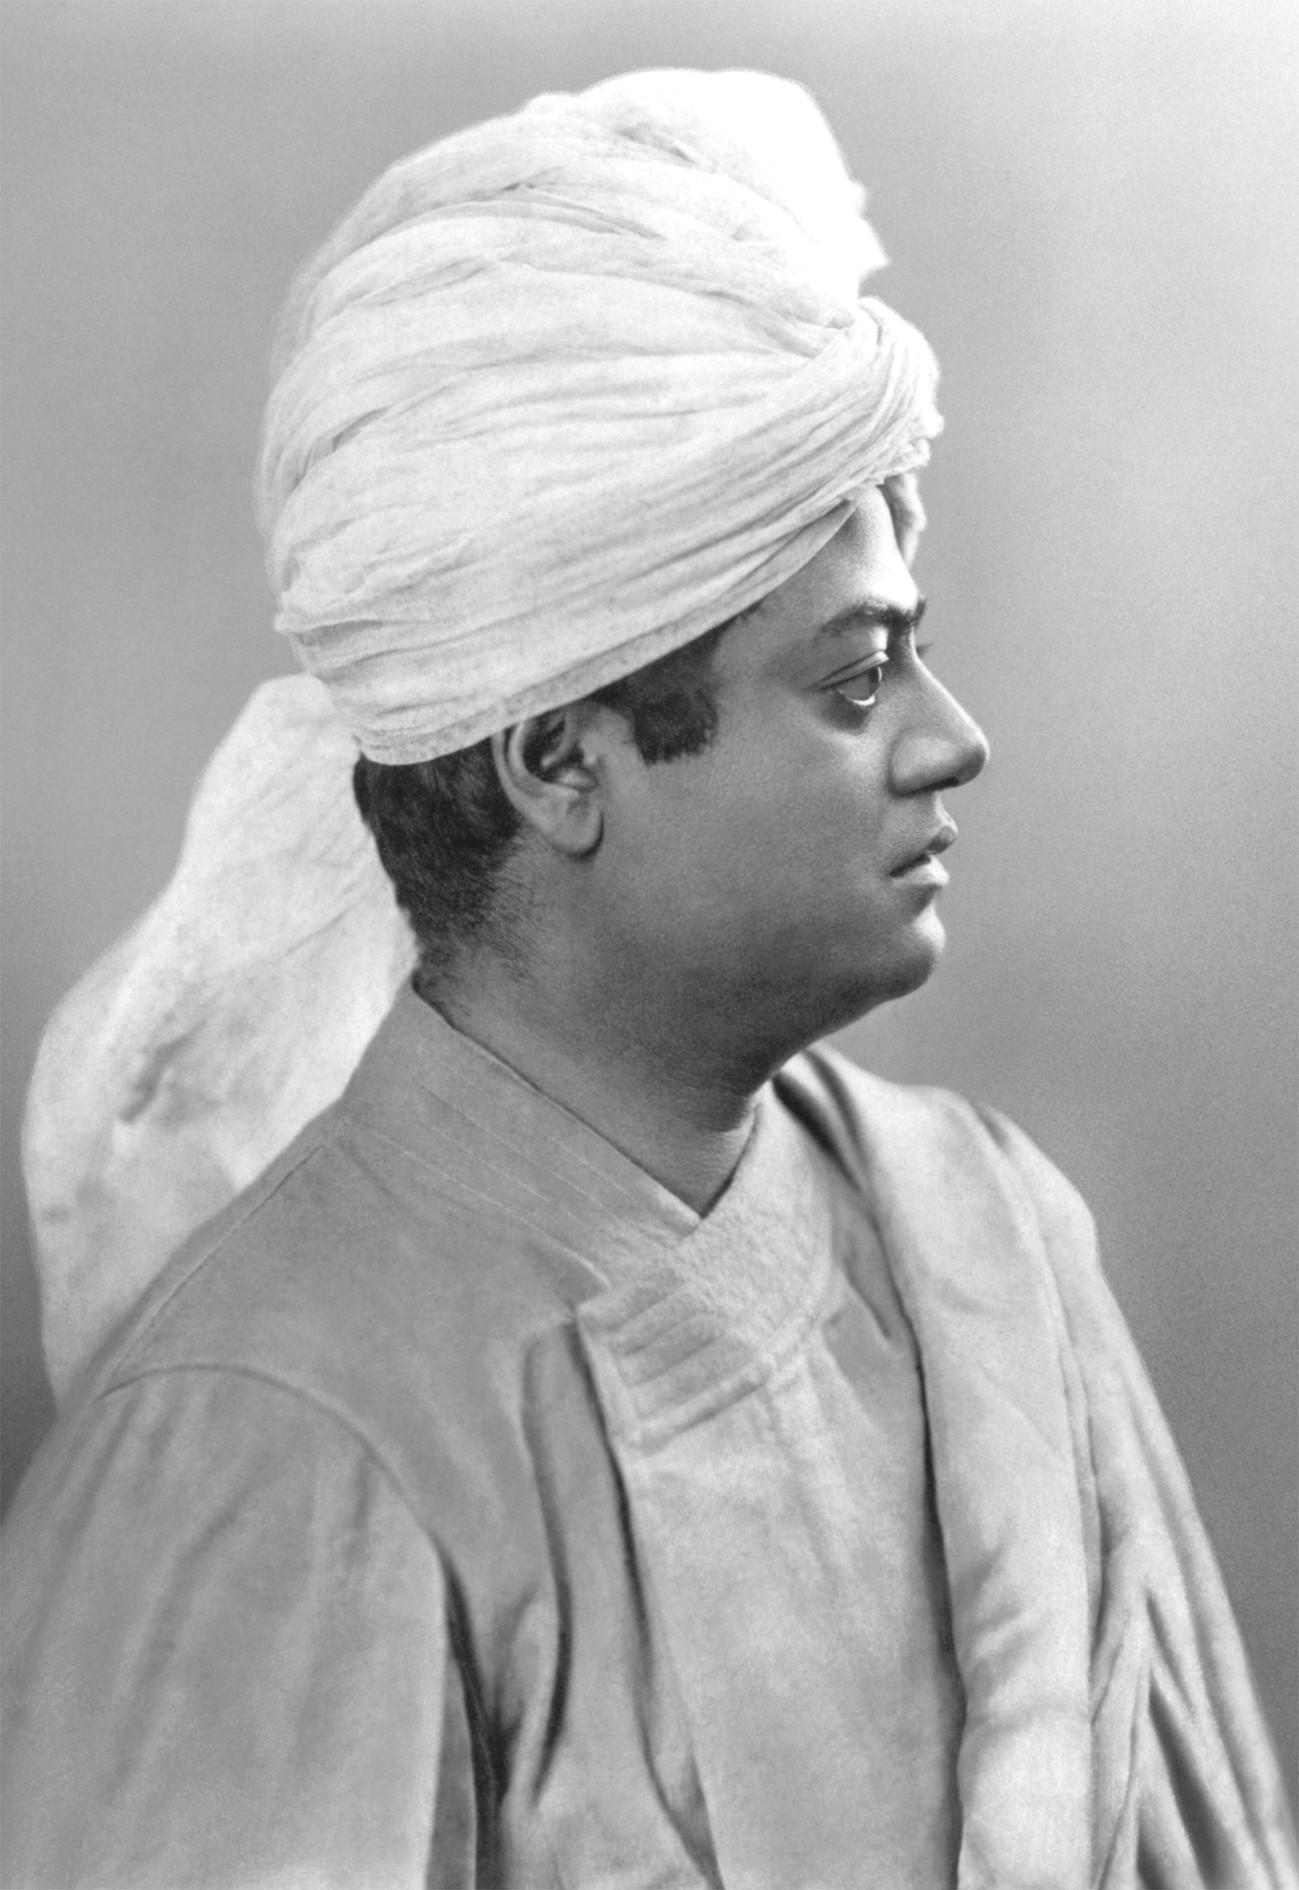
\includegraphics{images/vivekananda.jpg}
\end{center}

\chapter[ನನ್ನ ಜೀವನ ಮತ್ತು ಧ್ಯೇಯ]{ನನ್ನ ಜೀವನ ಮತ್ತು ಧ್ಯೇಯ\protect\footnote{\engfoot{Complete Works of Swami Vivekananda, Volume VIII, Page 73}}}

\begin{center}
(ಜನವರಿ ೨೭, ೧೯೦೦ ರಂದು ಅಮೆರಿಕಾದಲ್ಲಿ ಕ್ಯಾಲಿಫೋರ್ನಿಯಾದ ಪಸೆಡನಾದ ಷೇಕ್ಸ್‌ಪಿಯರ್ ಕ್ಲಬ್ಬಿನಲ್ಲಿ ನೀಡಿದ ಉಪನ್ಯಾಸ.)
\end{center}

ಈ ದಿನ ಪ್ರಾತಃಕಾಲ ನಾನು ಮಾತನಾಡಬೇಕಾದದ್ದು ವೇದಾಂತ ತತ್ತ್ವದ ವಿಚಾರ. ವಿಷಯವೇನೋ ತುಂಬಾ ಸ್ವಾರಸ್ಯವಾಗಿದೆ. ಆದರೆ ತುಂಬಾ ವಿಶಾಲ ಮತ್ತು ಕಷ್ಟ.

ತನ್ಮಧ್ಯೆ ಇಲ್ಲಿರುವ ನಿಮ್ಮ ಅಧ್ಯಕ್ಷರು, ಕೆಲವು ಮಹನೀಯರು ಮತ್ತು ಮಹಿಳೆಯರು, ನನ್ನ ಕೆಲಸದ ವಿಷಯವಾಗಿ, ನಾನು ಏನು ಮಾಡುತ್ತಿರುವೆನು ಎಂಬುದನ್ನು ಕುರಿತು ಹೇಳಬೇಕೆಂದು ಕೇಳಿಕೊಳ್ಳುತ್ತಲಿರುವರು. ಇಲ್ಲಿರುವ ಕೆಲವರಿಗೆ ಇದು ಸ್ವಾರಸ್ಯಕರವಾಗಿರಬಹುದು. ಆದರೆ ನನಗೆ ಈ ವಿಷಯದ ಮೇಲೆ ಅಷ್ಟು ಆಸಕ್ತಿಯಿಲ್ಲ. ನಿಜವಾಗಿ ಇದನ್ನು ನಾನು ನಿಮಗೆ ಹೇಗೆ ಹೇಳಬೇಕೋ ಅದೂ ಕೂಡ ಅಷ್ಟು ಚೆನ್ನಾಗಿ ಗೊತ್ತಿಲ್ಲ. ಏಕೆಂದರೆ ನನ್ನ ಜೀವನದಲ್ಲಿ ಇಂತಹ ವಿಷಯದ ಮೇಲೆ ಮಾತನಾಡುವುದು ಇದೇ ಮೊದಲು.

ಈಗ ಸಾಮಾನ್ಯ ರೀತಿಯಲ್ಲಿ ನಾನು ಏನು ಮಾಡುತ್ತಿರುವೆನು ಎಂದು ತಿಳಿದುಕೊಳ್ಳುವುದಕ್ಕಾಗಿ ನಿಮ್ಮನ್ನು ನಾನು ಕಲ್ಪನೆಯ ಮೂಲಕ ಭರತಖಂಡಕ್ಕೆ ಕರೆದುಕೊಂಡು\break ಹೋಗುವೆನು. ವಿಷಯವನ್ನು ಅಖಂಡವಾಗಿ, ವಿಸ್ತಾರವಾಗಿ ಹೇಳುವುದಕ್ಕೆ ಸಮಯವಿಲ್ಲ. ಇಷ್ಟು ಸ್ವಲ್ಪ ಕಾಲದಲ್ಲಿ ಅನ್ಯ ಜನಾಂಗದ ಜಟಿಲ ಸಮಸ್ಯೆಯನ್ನು ತಿಳಿದುಕೊಳ್ಳುವುದಕ್ಕೆ ಸಾಧ್ಯವೂ ಇಲ್ಲ. ಭರತಖಂಡ ಹೇಗಿರುವುದು ಎಂಬ ಚಿತ್ರವನ್ನು ಕೊಡುವುದಕ್ಕೆ ಪ್ರಯತ್ನಿಸುತ್ತೇನೆ. ಸದ್ಯಕ್ಕೆ ಅಷ್ಟೇ ಸಾಕು.

ಭರತಖಂಡ, ಕುಸಿದುಬಿದ್ದು ಹಾಳಾಗಿಹೋದ ಒಂದು ದೊಡ್ಡ ಮನೆಯಂತಿದೆ. ಇದನ್ನು ನೋಡಿದರೆ ಅದನ್ನು ಉತ್ತಮ ಸ್ಥಿತಿಗೆ ತರಲು ಅವಕಾಶವೇ ಇಲ್ಲವೆಂದು ತೋರುವುದು. ಇದೊಂದು ಮಾಯವಾದ ರಾಷ್ಟ್ರ, ಪಾಳುಬಿದ್ದ ರಾಷ್ಟ್ರ. ಆದರೆ ಸಾವಧಾನದಿಂದ ಇದನ್ನು ಪರೀಕ್ಷಿಸಿ. ಆಗ ಇದಕ್ಕಿಂತ ಸ್ವಲ್ಪ ಹೆಚ್ಚು ಕಾಣುವುದು. ಸತ್ಯಾಂಶವೇನೆಂದರೆ, ಎಲ್ಲಿಯವರೆಗೂ ತತ್ತ್ವ ಮತ್ತು ಆದರ್ಶಗಳಿಗೆ ಅಪಾಯ ತಗಲುವುದಿಲ್ಲವೋ, ಅವು ನಾಶವಾಗುವುದಿಲ್ಲವೋ, ಅಲ್ಲಿಯವರೆಗೆ ಹೊರಗೆ ಇರುವ ವ್ಯಕ್ತಿ, ಎಂದರೆ ಅವನ್ನು ವ್ಯಕ್ತಪಡಿಸುವವನು ಸಜೀವಿಯಾಗಿರುವನು. ಆ ವ್ಯಕ್ತಿಗೆ ಭರವಸೆ ಇದೆ. ನಿಮ್ಮ ಅಂಗಿ ಇಪ್ಪತ್ತು ವೇಳೆ ಕಳುವಾದರೂ ಅದರಿಂದ ನೀವು ಸಾಯುವುದಕ್ಕೆ ಕಾರಣವಿಲ್ಲ. ನೀವು ಮತ್ತೊಂದು ಹೊಸ ಅಂಗಿಯನ್ನು ಪಡೆಯಬಹುದು. ಅಂಗಿ ಅಷ್ಟು ಮುಖ್ಯವಲ್ಲ. ಶ‍್ರೀಮಂತರ ಆಸ್ತಿಯನ್ನು ಯಾರಾದರೂ ದರೋಡೆ ಮಾಡಿದರು ಎಂದರೆ ಅವರ ಸತ್ತ್ವಕ್ಕೆ ಕುಂದು ಬರುವುದಿಲ್ಲ. ಅದು ಮೃತ್ಯುವಲ್ಲ. ಅವರು ಬದುಕುತ್ತಾರೆ. ಈ ಧ್ಯೇಯದ ದೃಷ್ಟಿಯಿಂದ ನೋಡಿದರೆ ನಮಗೆ ಕಾಣುವುದು ಏನು? ಭರತಖಂಡ ಈಗ ಒಂದು ರಾಜಕೀಯವಾಗಿ ಸಶಕ್ತವಾದ ರಾಷ್ಟ್ರವಾಗಿಲ್ಲ; ಅದೊಂದು ಗುಲಾಮಗಿರಿಯಲ್ಲಿರುವ ಜನಾಂಗ, ಅವರ ಸರ್ಕಾರದಲ್ಲೇ ಅವರಿಗೆ ಯಾವ ಅಧಿಕಾರವೂ ಇಲ್ಲ, ಯಾವ ಸ್ವಾತಂತ್ರ್ಯವೂ ಇಲ್ಲ. ಮೂವತ್ತು ಕೋಟಿ ಗುಲಾಮರು ಅವರು. ಮತ್ತೇನೂ ಅಲ್ಲ! ಭಾರತೀಯರ ತಿಂಗಳ ಸಾಧಾರಣ ಸಂಪಾದನೆ ಎರಡು ಷಿಲಿಂಗು. ಇರುವ ಬಹುಜನರ ಸಾಧಾರಣ ಜೀವನದ ಮಟ್ಟ ಉಪವಾಸಕ್ಕೆ ಸಮೀಪದಲ್ಲಿರುವುದು. ಆದಕಾರಣ ಸ್ವಲ್ಪ ಸಂಪಾದನೆ ಕಡಿಮೆಯಾದರೂ ಲಕ್ಷಾಂತರ ಜನರು ಸಾಯುವರು. ಸ್ವಲ್ಪ ಬರಗಾಲ ಬಂದರೂ ಸಾವು ನಿಶ್ಚಯ. ಈ ದೃಷ್ಟಿಯಿಂದ ನೋಡಿದರೂ ಭರತಖಂಡದಲ್ಲಿ\break ಕಾಣುವುದು ನಾಶ, ನೆಚ್ಚಿಗೆ ಇಲ್ಲದ ನಾಶ.

ಭಾರತೀಯ ಜನಾಂಗ ಎಂದಿಗೂ ಐಶ್ವರ್ಯವನ್ನೇ ತನ್ನ ಜೀವನದ ಗುರಿ ಮಾಡಿಕೊಂಡಿರಲಿಲ್ಲವೆಂಬುದು ನಮಗೆ ಕಾಣುವುದು. ಅವರು ಬೇಕಾದಷ್ಟು ಐಶ್ವರ್ಯವನ್ನು ಪಡೆದರೂ, ಉಳಿದ ಎಲ್ಲಾ ರಾಷ್ಟ್ರಗಳಿಗಿಂತಲೂ ಹೆಚ್ಚು ಪಡೆದಿದ್ದರೂ, ಜನಾಂಗದ ಧ್ಯೇಯ ಐಶ್ವರ್ಯವಲ್ಲ. ಹಲವು ಶತಮಾನದವರೆಗೆ ಈ ಜನಾಂಗ ಬಲಾಢ್ಯವಾಗಿತ್ತು. ಆದರೂ ಅದು ಅಧಿಕಾರಕ್ಕೆ ನಿಲ್ಲಲಿಲ್ಲ; ಆಕ್ರಮಣಕ್ಕಾಗಿ, ದೇಶವನ್ನು ಬಿಟ್ಟು ಹೋದದ್ದು ಕಾಣುವುದಿಲ್ಲ. ಅವರು ತಮ್ಮ ದೇಶದಲ್ಲೇ ತೃಪ್ತರಾಗಿದ್ದರು. ಮತ್ತೊಬ್ಬರೊಂದಿಗೆ ಹೋರಾಡಲಿಲ್ಲ. ಭಾರತೀಯ ಜನಾಂಗ ಸಾಮ್ರಾಜ್ಯ ಕೀರ್ತಿಯ ಆದರ್ಶವನ್ನು ಇಟ್ಟುಕೊಳ್ಳಲಿಲ್ಲ. ದ್ರವ್ಯ ಮತ್ತು ಕೀರ್ತಿ ಜನಾಂಗದ ಗುರಿಯಾಗಿರಲಿಲ್ಲ.

ಹಾಗಾದರೆ ಏನು? ಅವರ ಆದರ್ಶ ಸರಿಯೆ ಅಥವಾ ತಪ್ಪೆ? ಅದನ್ನಲ್ಲ ನಾವು ವಿಮರ್ಶಿಸುತ್ತಿರುವುದು. ಆ ದೇಶ ಉಳಿದ ಎಲ್ಲಾ ಮಾನವ ಸಂತಾನಕ್ಕಿಂತಲೂ ಹೆಚ್ಚಾಗಿ, ಈ ಜೀವನ ಅನಿತ್ಯವೆಂಬುದನ್ನು ನಂಬಿತ್ತು, ದೃಢವಾಗಿ ನಂಬಿತ್ತು. ನಿತ್ಯವಾದುದೇ ದೇವರು; ಏನಾದರೂ ಆಗಲಿ ಅವರು ದೇವರನ್ನು ಬಿಡಲಿಲ್ಲ. ಅವರು ಹೀನಸ್ಥಿತಿಯಲ್ಲಿದ್ದಾಗ ಮೊದಲು ಅವರ ದೃಷ್ಟಿ ಧರ್ಮದ ಕಡೆಗೆ ತಿರುಗಿತು. ಹಿಂದೂ ಧಾರ್ಮಿಕವಾಗಿ ಕುಡಿಯುವನು, ಧಾರ್ಮಿಕವಾಗಿ ಮಲಗುವನು, ಧಾರ್ಮಿಕವಾಗಿ ನಡೆಯುವನು, ಧಾರ್ಮಿಕವಾಗಿ ಮದುವೆಯಾಗುವನು, ಧಾರ್ಮಿಕವಾಗಿ ದರೋಡೆ ಮಾಡುವನು!

ಇಂತಹ ದೇಶವನ್ನು ನೀವು ಎಂದಾದರೂ ನೋಡಿರುವಿರಾ! ನೀವು ಒಂದು ದರೋಡೆಕಾರರ ಗುಂಪನ್ನು ಕೂಡಿಸಬೇಕಾದರೆ, ಅದರ ನಾಯಕ ಯಾವುದಾದರೂ ಧರ್ಮವನ್ನು ಬೋಧಿಸಬೇಕು. ಯಾವುದಾದರೂ ಥಳುಕಿನ ತತ್ತ್ವವನ್ನು ವಿವರಿಸಬೇಕು. ದೇವರ ಸಮೀಪಕ್ಕೆ ಅತಿ ನೇರವಾಗಿ, ಶೀಘ್ರವಾಗಿ ಈ ಮಾರ್ಗ ಕರೆದೊಯ್ಯುವುದು ಎಂದು ಹೇಳಬೇಕು. ಆಗ ಅವನಿಗೆ ಅನುಯಾಯಿಗಳು ಸಿಕ್ಕುವರು. ಇಲ್ಲದಿದ್ದರೆ ಇಲ್ಲ. ಜನಾಂಗದ ಜೀವಾಳ, ಜನಾಂಗದ ಕರ್ತವ್ಯವಿರುವುದು ಧರ್ಮದಲ್ಲಿ ಎನ್ನುವುದನ್ನು ಇದು ತೋರುವುದು. ಅದು ಇನ್ನೂ ನಾಶವಾಗಿಲ್ಲ. ಆದಕಾರಣ ಜನಾಂಗ ಜೀವಿಸಿರುವುದು.

ರೋಮ್ ದೇಶವನ್ನು ನೋಡಿ, ರೋಮಿನ ಆದರ್ಶ ಸಾಮ್ರಾಜ್ಯ ಶಕ್ತಿ. ಇದನ್ನು ಮುಟ್ಟಿದೊಡನೆಯೇ ರೋಮ್ ನುಚ್ಚುನೂರಾಯಿತು, ಮಾಯವಾಯಿತು. ಗ್ರೀಸಿನ ಸಂದೇಶ ಬೌದ್ಧಿಕ ಪ್ರಗತಿ. ಅದನ್ನು ಮುಟ್ಟಿದೊಡನೆಯೇ ಗ್ರೀಸ್ ಮಾಯವಾಯಿತು. ಹೀಗೆಯೇ ವರ್ತಮಾನಕಾಲದಲ್ಲೂ ಸ್ಪೇನ್ ಮತ್ತು ಇತರ ದೇಶಗಳೂ ಕೂಡ. ಜಗತ್ತಿಗೆ ಕೊಡುವುದಕ್ಕೆ ಪ್ರತಿಯೊಂದು ಜನಾಂಗಕ್ಕೂ ಒಂದು ಸಂದೇಶವಿದೆ. ಎಲ್ಲಿಯವರೆವಿಗೂ ಆ ಸಂದೇಶಕ್ಕೆ ಅಪಾಯ ತಗಲುವುದಿಲ್ಲವೋ ಅಲ್ಲಿಯವರೆಗೂ ಎಷ್ಟು ಕಷ್ಟ ಬಂದರೂ ಆ ಜನಾಂಗ ಬಾಳುವುದು. ಎಂದು ಅವರ ಸಂದೇಶ ನಾಶವಾಗುವುದೋ ಅಂದು ಆ ಜನಾಂಗ\break ನಾಶವಾಗುವುದು.

ಭಾರತೀಯ ಸತ್ತ್ವಕ್ಕೆ ಇನ್ನೂ ಭಂಗ ಬಂದಿಲ್ಲ. ಭಾರತೀಯರು ಅದನ್ನು ತೊರೆದಿಲ್ಲ. ಅವರಲ್ಲಿ ಎಷ್ಟೇ ಮೂಢಭಕ್ತಿಯಿದ್ದರೂ ಆ ಸತ್ತ್ವ ಇನ್ನೂ ದೃಢವಾಗಿರುವುದು. ಅಲ್ಲಿ ಘೋರವಾದ ಮೂಢನಂಬಿಕೆಗಳಿವೆ. ಕೆಲವು ಅತ್ಯಂತ ಅಸಹ್ಯಕರವಾದವು; ಆದರೂ ಚಿಂತೆಯಿಲ್ಲ. ಜನಾಂಗದ ಆದರ್ಶ, ಅದರ ಜೀವನಾಡಿ, ಇನ್ನೂ ಮಿಡಿಯುತ್ತಿದೆ.

ಭಾರತೀಯರು ಅನ್ಯರನ್ನು ಗೆಲ್ಲುವ ಜನಾಂಗವಾಗಲಾರರು, ಎಂದೆಂದಿಗೂ ಆಗಲಾರರು. ಅದೆಂದಿಗೂ ಪ್ರಚಂಡ ರಾಜಕೀಯ ಶಕ್ತಿ ಆಗಲಾರದು. ಅದು ಅವರ ಕರ್ತವ್ಯವಲ್ಲ. ಜನಾಂಗದ ಐಕ್ಯತೆಗೆ ಭಾರತೀಯರು ಹಾಡಬೇಕಾದ ಸ್ವರ ಅದಲ್ಲ. ಆದರೆ ಅವರ ಗುರಿ ಯಾವುದು? ದೇವರು, ದೇವರೊಬ್ಬನೆ. ಮೃತ್ಯು ಜನರನ್ನು ಹಿಡಿದುಕೊಂಡಿರುವಂತೆ ಅವರು ಅದನ್ನು ಗಟ್ಟಿಯಾಗಿ ಹಿಡಿದುಕೊಂಡಿರುವರು. ಇನ್ನೂ ಅಲ್ಲಿ ನೆಚ್ಚಿಗೆಗೆ ಅವಕಾಶವಿದೆ.

ಅಲ್ಲಿ ದಾರಿದ್ರ್ಯವಿದೆ, ದುಃಖವಿದೆ. ಆದರೆ ಅದರಿಂದ ಬಾಧಕವಿಲ್ಲ. ವ್ಯಕ್ತಿ ಬದುಕಿರುವನು. ಅದರಿಂದ ನೆಚ್ಚಿಗೆ ಇದೆ ಎಂಬ ನಿರ್ಣಯಕ್ಕೆ, ನಾವು ವಿಮರ್ಶೆಯ ಮೂಲಕ\break ಬರಬಹುದು.

ಹಾಗಾದರೆ ನೋಡಿ! ದೇಶದಲ್ಲೆಲ್ಲಾ ಆಗುತ್ತಿರುವ ಧಾರ್ಮಿಕ ಚಟುವಟಿಕೆಯನ್ನು ಗಮನಿಸಿ, ಭರತಖಂಡದಲ್ಲಿ ಹೊಸ ಪಂಥ ಹುಟ್ಟಿದ ವರುಷವೇ ನನಗೆ ಜ್ಞಾಪಕವಿಲ್ಲ. ಪ್ರವಾಹ ವೇಗವಾದಷ್ಟೂ ಸುಳಿಗಳು ಹೆಚ್ಚು. ಪಂಥ ಅವನತಿಯ ಗುರುತಲ್ಲ, ಜೀವದ ಚಿಹ್ನೆ ಅದು. ನಮ್ಮಲ್ಲಿ ಪ್ರತಿಯೊಬ್ಬರೂ ಒಂದು ಪಂಥವಾಗುವವರೆಗೆ ಪಂಥಗಳು ಹೆಚ್ಚುತ್ತಾ ಹೋಗಲಿ, ಅವುಗಳ ವಿಷಯವಾಗಿ ನಾವು ವ್ಯಾಜ್ಯವಾಡಬೇಕಾಗಿಲ್ಲ.

ಈಗ ನಿಮ್ಮ ದೇಶವನ್ನು ತೆಗೆದುಕೊಳ್ಳಿ. ನಾನು ಆಕ್ಷೇಪಣೆಗೆ ಹೇಳುವುದಿಲ್ಲ. ಇಲ್ಲಿನ ಸಾಮಾಜಿಕ ನಿಯಮಗಳು, ರಾಜಕೀಯ ಸ್ಥಿತಿ, ಎಲ್ಲಾ ಮಾನವನ ಇಹ ಜನ್ಮದ ಸ್ಥಿತಿಯನ್ನು ಉತ್ತಮಪಡಿಸುವುದಕ್ಕಾಗಿ ರಚಿಸಲ್ಪಟ್ಟಿವೆ. ಪ್ರಪಂಚದಲ್ಲಿ ಇರುವತನಕ ಒಬ್ಬನು ಸುಖವಾಗಿ ಇರಬಹುದು. ನಿಮ್ಮ ರಸ್ತೆಗಳನ್ನು ನೋಡಿ, ಎಷ್ಟು ಶುಭ್ರವಾಗಿವೆ. ನಗರಗಳು ಎಷ್ಟು ಸುಂದರವಾಗಿವೆ. ಮನುಷ್ಯ ಎಷ್ಟು ವಿಧದಲ್ಲಿ ಹಣ ಸಂಪಾದನೆ ಮಾಡಬಹುದು, ಸುಖವನ್ನು ಎಷ್ಟು ವಿಧದಲ್ಲಿ ಪಡೆಯಬಹುದು. ಆದರೆ ಇಲ್ಲಿ ಒಬ್ಬನು, “ನೋಡಿ, ನಾನು ಮರದ ಕೆಳಗೆ ಕುಳಿತು ಧ್ಯಾನಮಾಡುತ್ತೇನೆ. ಕೆಲಸ ಮಾಡುವುದಿಲ್ಲ” ಎಂದರೆ ಅವನು ಜೈಲಿಗೆ ಹೋಗಬೇಕಾಗುವುದು. ನೋಡಿದಿರಾ? ಅವನಿಗೆ ತನ್ನ ಬಯಕೆಯನ್ನು ಈಡೇರಿಸಿಕೊಳ್ಳುವುದಕ್ಕೆ ಆಸ್ಪದವೇ ಇಲ್ಲ, ಯಾವ ದಾರಿಯೂ ಇಲ್ಲ. ಉಳಿದವರಂತೆ ತಾನು ಆಚರಿಸಿದರೆ ಅವನು ಈ ಸಮಾಜದಲ್ಲಿ ಬಾಳಬಹುದು. ಈ ಜೀವನದ ಸೌಖ್ಯವನ್ನು ಅನುಭವಿಸುವ ಗಲಭೆಯಲ್ಲಿ ತಾನು ಸೇರಬೇಕು. ಇಲ್ಲದೆ ಇದ್ದರೆ ಅವನು ಸಾಯುವನು.

ಈಗ ನಾವು ಪುನಃ ಭರತಖಂಡಕ್ಕೆ ಹೋಗೋಣ. ಅಲ್ಲಿ ಒಬ್ಬನು, “ಬೆಟ್ಟದಮೇಲೆ ಹೋಗಿ ಕುಳಿತುಕೊಂಡು ನಾನು ಬದುಕಿರುವ ಪರಿಯಂತರವೂ ಮೂಗಿನ ಕೊನೆಯನ್ನೇ ನೋಡುತ್ತಾ ಧ್ಯಾನಮಾಡುವೆ” ಎಂದರೆ ಎಲ್ಲರೂ ಅವನನ್ನು, “ಹೋಗಪ್ಪ, ದೇವರು ನಿನಗೆ ಒಳ್ಳೆಯದು ಮಾಡಲಿ” ಎನ್ನುವರು. ಅವನು ಒಂದು ಮಾತನ್ನೂ ಆಡಬೇಕಾಗಿಲ್ಲ. ಅವನಿಗೆ ಯಾರಾದರೂ ಒಂದು ಚೂರು ರೊಟ್ಟಿಯನ್ನು ತಂದುಕೊಡುವರು. ಅವನು ಆರೋಗ್ಯದಿಂದ ಇರುವನು. ಆದರೆ ಒಬ್ಬ, “ನೋಡಿ, ಈ ಪ್ರಪಂಚದ ಸೌಖ್ಯವನ್ನು ನಾನು ಸ್ವಲ್ಪ ಅನುಭವಿಸುತ್ತೇನೆ” ಎಂದರೆ ಎಲ್ಲರೂ ನಿರಾಕರಿಸುವವರೆ!

ಎರಡು ದೇಶಗಳ ಆದರ್ಶಗಳೂ ಅನ್ಯಾಯವೆಂದು ನಾನು ಹೇಳುತ್ತೇನೆ. ಇಲ್ಲಿ ಒಬ್ಬನು ಆಶಿಸಿದರೆ ಕುಳಿತುಕೊಂಡು ಮೂಗಿನ ಕೊನೆಯನ್ನು ಏಕೆ ನೋಡಬಾರದು? ಇದಕ್ಕೆ ಕಾರಣ ನನಗೆ ಗೊತ್ತಿಲ್ಲ. ಬಹುಪಾಲು ಜನರು ಏನನ್ನು ಮಾಡುತ್ತಾರೆಯೋ ಅದನ್ನೇ ಏತಕ್ಕೆ ಎಲ್ಲರೂ ಮಾಡಬೇಕು? ನನಗೆ ಇದಕ್ಕೆ ಕಾರಣ ಗೊತ್ತಾಗುವುದಿಲ್ಲ.

ಭರತಖಂಡದಲ್ಲಿ ಏತಕ್ಕೆ ಒಬ್ಬನು ಈ ಪ್ರಪಂಚದ ಒಳ್ಳೆಯ ವಸ್ತುವನ್ನು ಇಟ್ಟುಕೊಂಡು ದುಡ್ಡು ಮಾಡಬಾರದು? ನೋಡಿ ಬಲಾತ್ಕಾರದಿಂದ ಹೇಗೆ ಕೋಟ್ಯಂತರ ಜನರು ತಮಗೆ ವಿರೋಧವಾದ ಅಭಿಪ್ರಾಯವನ್ನು ಸ್ವೀಕರಿಸುವಂತೆ ಮಾಡಿರುವರು! ಇದು ಋಷಿಗಳ ದಬ್ಬಾಳಿಕೆ, ಇದೇ ಮಹಾತ್ಮರ ದಬ್ಬಾಳಿಕೆ, ಧಾರ್ಮಿಕ ದಬ್ಬಾಳಿಕೆ, ಬುದ್ಧಿವಂತರ ದಬ್ಬಾಳಿಕೆ, ಜ್ಞಾಪಕದಲ್ಲಿಡಿ! ತಿಳಿದವರ ದಬ್ಬಾಳಿಕೆ, ತಿಳಿಯದವರ ದಬ್ಬಾಳಿಕೆಗಿಂತ ಘೋರವಾದದ್ದು. ಪಂಡಿತರು, ಬುದ್ಧಿವಂತರು, ಮತ್ತೊಬ್ಬರಮೇಲೆ ತಮ್ಮ ಅಭಿಪ್ರಾಯವನ್ನು ಬಲಾತ್ಕರಿಸುವುದಕ್ಕೆ, ಪಾಮರರು ಪಾರಾಗಲು ಅಸಾಧ್ಯವಾದ ಸಾವಿರಾರು ಬಂಧನಗಳನ್ನು ಅವರ ಮಾರ್ಗದಲ್ಲಿ ತಂದೊಡ್ಡಬಲ್ಲರು.

ಇದು ಇಲ್ಲಿಗೇ ಕೊನೆಗಾಣಬೇಕೆಂದು ನಾನು ಹೇಳುತ್ತೇನೆ. ಒಬ್ಬ ಆಧ್ಯಾತ್ಮಿಕ ಮಹಾಪುರುಷನ ತಯಾರಿಕೆಗಾಗಿ ಲಕ್ಷೋಪಲಕ್ಷ ಜೀವಿಗಳನ್ನು ಬಲಿಗೊಡುವುದರಿಂದ ಪ್ರಯೋಜನವಿಲ್ಲ. ಎಲ್ಲಿ ಆಧ್ಯಾತ್ಮಿಕ ವೀರರೂ ಉದ್ಭವಿಸಿ, ಉಳಿದವರೂ ಸುಖವಾಗಿರುವರೋ,\break ಸಂತೋಷವಾಗಿರುವರೊ, ಅಂತಹ ಸಮಾಜವಿದ್ದರೆ ಅದು ಒಳ್ಳೆಯದು. ಆದರೆ ಲಕ್ಷೋಪಲಕ್ಷ ಜೀವಿಗಳು ಅದಕ್ಕಾಗಿ ಆಹುತಿಯಾಗಬೇಕಾದರೆ ಅದು ಅನ್ಯಾಯ. ಜಗದ ಉದ್ಧಾರಕ್ಕಾಗಿ ಮಹಾತ್ಮನೊಬ್ಬನು ಕಷ್ಟವನ್ನು ಅನುಭವಿಸುವುದು ಒಳ್ಳೆಯದು.

ಪ್ರತಿಯೊಂದು ದೇಶದಲ್ಲೂ ನೀವು ಅವರ ವಿಧಾನದಲ್ಲಿಯೇ ಕೆಲಸ ಮಾಡಬೇಕಾಗಿದೆ, ಪ್ರತಿಯೊಬ್ಬರೊಂದಿಗೂ ನೀವು ಅವರವರ ಭಾಷೆಯಲ್ಲೇ ಮಾತನಾಡಬೇಕಾಗಿದೆ. ಈಗಿನ ಅಮೆರಿಕಾ ಅಥವಾ ಇಂಗ್ಲೆಂಡಿನ ಜನರಿಗೆ ಧರ್ಮವನ್ನು ಬೋಧಿಸಬೇಕಾದರೆ ರಾಜಕೀಯ ವಿಧಾನದಲ್ಲಿಯೇ ಅದನ್ನು ಮಾಡಬೇಕಾಗಿದೆ. ಸಂಸ್ಥೆ, ಮಂಡಲಿ ಮುಂತಾದುವನ್ನು ಮಾಡಬೇಕು, ಒಬ್ಬ ಅಧ್ಯಕ್ಷನನ್ನು ಚುನಾವಣೆ ಮಾಡಬೇಕು. ಏಕೆಂದರೆ ಪಾಶ್ಚಾತ್ಯ ಜನರ ಭಾಷೆ ಅದು, ಮಾರ್ಗ ಅದು. ಅದಲ್ಲದೆ ಇಂಡಿಯಾದೇಶದಲ್ಲಿ ನೀವು ರಾಜಕೀಯ ವಿಷಯವನ್ನು ಮಾತನಾಡಬೇಕಾದರೆ ಧಾರ್ಮಿಕ ಭಾಷೆಯಲ್ಲಿ ಮಾತನಾಡಬೇಕಾಗಿದೆ. ಅವರಿಗೆ ನೀವು ಹೀಗೆ ಏನಾದರೂ ಹೇಳಬೇಕು: “ಪ್ರತಿದಿನವೂ ತಮ್ಮ ಮನೆಯನ್ನು ಗುಡಿಸುವವನಿಗೆ ಇಂತಹ ಪುಣ್ಯ ಬರುವುದು. ಅವನು ಸ್ವರ್ಗಕ್ಕೆ ಹೋಗುವನು, ಅಥವಾ ದೇವರ ಹತ್ತಿರಕ್ಕೆ ಬರುವನು.” ಹೀಗೆ ಹೇಳದೆ ಹೋದರೆ ಅವರು ಕೇಳುವುದೇ ಇಲ್ಲ. ಇದು ಒಂದು ಭಾಷೆಯ ಪ್ರಶ್ನೆ. ಮಾಡಿದ ಕೆಲಸವೇನೋ ಒಂದೆ. ಆದರೆ ಪ್ರತಿಯೊಂದು ಜನಾಂಗದವರೊಂದಿಗೂ, ಅವರ ಹೃದಯಕ್ಕೆ ನಾಟಬೇಕಾದರೆ, ಅವರ ಭಾಷೆಯಲ್ಲಿ ಮಾತನಾಡಬೇಕಾಗಿದೆ. ಅದು ನ್ಯಾಯ; ಅದನ್ನು ನಾವು ಅಲ್ಲಗಳೆಯಬೇಕಾಗಿಲ್ಲ.

ನಾನು ಸೇರಿರುವ ಪಂಥದಲ್ಲಿ ನಮ್ಮನ್ನು ಸಂನ್ಯಾಸಿಗಳೆಂದು ಕರೆಯುತ್ತಾರೆ. ಸಂನ್ಯಾಸಿ ಎಂದರೆ ತ್ಯಾಗ ಮಾಡಿರುವವನು ಎಂದು ಅರ್ಥ. ಇದು ಬಹಳ ಪುರಾತನ ಸಂಸ್ಥೆ. ಕ್ರಿ.ಪೂ. ೫೬೦ರಲ್ಲಿ ಇದ್ದ ಬುದ್ಧದೇವನು ಕೂಡ ಈ ಪಂಗಡಕ್ಕೆ ಸೇರಿದ್ದನು. ಈ ಪಂಗಡದ ಹಲವು ಸುಧಾರಕರಲ್ಲಿ ಅವನೊಬ್ಬನು ಅಷ್ಟೆ. ಇದು ಅಷ್ಟು ಪುರಾತನವಾಗಿತ್ತು! ಪ್ರಪಂಚದ ಅತಿ ಪುರಾತನ ಗ್ರಂಥವಾದ ವೇದಗಳಲ್ಲಿಯೂ ಇದರ ಪ್ರಸ್ತಾಪವಿದೆ. ಹಿಂದಿನ ಕಾಲದ ಭರತಖಂಡದಲ್ಲಿ ಪ್ರತಿಯೊಬ್ಬ ಸ್ತ್ರೀಪುರುಷರೂ ಕೊನೆಗಾಲದಲ್ಲಿ ಸಮಾಜದಿಂದ ಹೊರಗೆ ಹೋಗಿ ತಮ್ಮ ಮುಕ್ತಿಚಿಂತನೆ ಮತ್ತು ಭಗವಂತನ ಧ್ಯಾನವನ್ನು ಮಾತ್ರ ಮಾಡಬೇಕೆಂಬ ಒಂದು ನಿಯಮವಿತ್ತು. ಸಾವೆಂಬ ಮಹಾ ಘಟನೆಗೆ ಅಣಿಯಾಗುವುದೇ ಇದರ ಉದ್ದೇಶ. ಆದಕಾರಣವೇ ವೃದ್ದರು ಅಂದಿನ ಕಾಲದಲ್ಲಿ ಸಂನ್ಯಾಸಿಗಳಾಗುತ್ತಿದ್ದರು. ನಂತರ ಯುವಕರು ಕೂಡ ಪ್ರಪಂಚವನ್ನು ತೊರೆಯಲು ಪ್ರಾರಂಭಿಸಿದರು. ಯುವಕರು ಚಟುವಟಿಕೆಯ ಸ್ವಭಾವದವರು. ಆದಕಾರಣ ಅವರು ಮರದ ಕೆಳಗೆ ಕುಳಿತುಕೊಂಡು ದಿನವೆಲ್ಲಾ ತಮ್ಮ ಸಾವಿನ ವಿಚಾರವನ್ನು ಆಲೋಚಿಸುವುದಕ್ಕೆ ಸಾಧ್ಯವಾಗಲಿಲ್ಲ. ಅವರು ಪ್ರಚಾರ ಮತ್ತು ಹೊಸ ಸಂಪ್ರದಾಯದ ಸ್ಥಾಪನೆ ಮುಂತಾದುವುಗಳಿಗೆ ಕೈಯಿಟ್ಟರು. ಬುದ್ಧನು ಇನ್ನೂ ಚಿಕ್ಕವನಾಗಿದ್ದುದರಿಂದ ಸುಧಾರಣೆಯನ್ನು ಕೈಕೊಂಡನು. ಅವನೇನಾದರೂ ವೃದ್ಧನಾಗಿದ್ದರೆ ಮೂಗಿನ ಕೊನೆಯನ್ನೇ ನೋಡುತ್ತಾ ಶಾಂತವಾಗಿ ಸಾಯುತ್ತಿದ್ದನು.

ಈ ಪಂಥ ಒಂದು ಚರ್ಚ್ ಅಲ್ಲ. ಇದಕ್ಕೆ ಸೇರಿದವರು ಪೂಜಾರಿಗಳಲ್ಲ. ಪೂಜಾರಿಗಳಿಗೂ ಸಂನ್ಯಾಸಿಗಳಿಗೂ ಎಷ್ಟೋ ಅಂತರವಿದೆ! ಭರತಖಂಡದಲ್ಲಿ ಪೌರೋಹಿತ್ಯವು\break ಸಮಾಜದ ಉಳಿದ ಎಲ್ಲಾ ಕಾರ್ಯರಂಗಗಳಂತೆಯೇ ವಂಶಾನುಗತವಾಗಿ ಬಂದುದು. ಬಡಗಿಯ ಮಗ ಬಡಗಿಯಾಗುವಂತೆ, ಕಮ್ಮಾರನ ಮಗ ಕಮ್ಮಾರನಾಗುವಂತೆ, ಪುರೋಹಿತನ ಮಗ ಪುರೋಹಿತನಾಗುವನು. ಪುರೋಹಿತನು ಯಾವಾಗಲೂ ಮದುವೆಯಾಗಿರಬೇಕು. ಒಬ್ಬನಿಗೆ ಹೆಂಡತಿ ಇದ್ದ ಹೊರತು ಅವನು ಪೂರ್ಣನಾಗಲಾರ ಎಂಬುದು ಹಿಂದುವಿನ ಅಭಿಪ್ರಾಯ. ಮದುವೆಯಾಗದವನಿಗೆ ಯಾವ ಕರ್ಮವನ್ನು ಮಾಡುವುದಕ್ಕೂ\break ಅಧಿಕಾರವಿಲ್ಲ.

ಸಂನ್ಯಾಸಿಗಳಿಗೆ ಯಾವ ಆಸ್ತಿಪಾಸ್ತಿಗಳೂ ಇಲ್ಲ. ಅವರು ಮದುವೆಯಾಗುವುದಿಲ್ಲ. ಇದಕ್ಕಿಂತ ಹೆಚ್ಚಾಗಿ ಯಾವ ವ್ಯವಸ್ಥೆಯೂ ಇಲ್ಲ. ಇರುವ ಒಂದು ಸಂಬಂಧವೇ ಗುರು ಶಿಷ್ಯನಿಗೆ ಇರುವ ಸಂಬಂಧ. ಇದು ಹಿಂದುಗಳ ವೈಶಿಷ್ಟ್ಯ. ಗುರುವೆಂದರೆ ಕೇವಲ ನನಗೆ ಕಲಿಸುವುದಕ್ಕಾಗಿ ಒಬ್ಬ ಬರುವನು, ನಾನು ಅದಕ್ಕೆ ಇಷ್ಟೊಂದು ಹಣ ಕೊಡುವೆನು – ಇಲ್ಲಿಗೇ ಕೊನೆಗಾಣುವುದಲ್ಲ. ಭರತಖಂಡದಲ್ಲಿ ಇದು ಒಬ್ಬನನ್ನು ದತ್ತು ತೆಗೆದುಕೊಂಡಂತೆ. ಗುರು ನನ್ನ ತಂದೆಗಿಂತ ಹೆಚ್ಚು. ನಾನು ನಿಜವಾಗಿಯೂ ಪ್ರತಿಯೊಂದು ರೀತಿಯಲ್ಲೂ ಅವನ ಮಗ. ತಂದೆಗಿಂತ ಮೊದಲು ಗುರುವಿಗೆ ಭಕ್ತಿ, ಗೌರವಗಳನ್ನು ತೋರುವುದು ನನ್ನ ಕರ್ತವ್ಯ. ಏಕೆಂದರೆ ತಂದೆ ನನಗೆ ಈ ದೇಹವನ್ನು ಕೊಟ್ಟನು. ಆದರೆ ಗುರು ಮುಕ್ತಿಮಾರ್ಗವನ್ನು ತೋರಿದವನು. ಆದಕಾರಣವೇ ನನ್ನ ತಂದೆಗಿಂತಲೂ ಗುರು ಹೆಚ್ಚು. ಇದೊಂದೇ ಇರುವ ವ್ಯವಸ್ಥೆ. ಈ ಸಂಬಂಧವನ್ನು, ಗುರುವಿನ ವಿಷಯದಲ್ಲಿ ಪ್ರೇಮ ಗೌರವಗಳನ್ನು ಜೀವನದ ಕೊನೆಯವರೆಗೂ ಉಳಿಸಿಕೊಳ್ಳುತ್ತೇನೆ. ನಾನು ಶಿಷ್ಯರನ್ನು ಸ್ವೀಕರಿಸುತ್ತೇನೆ. ಕೆಲವು ವೇಳೆ ಗುರು ಯುವಕನಾಗಿರುವನು, ಶಿಷ್ಯ ವೃದ್ಧನಾಗಿರುವನು. ಇದನ್ನು ಗಮನಿಸಬೇಕಾಗಿಲ್ಲ; ಅವನು ಮಗ; ನನ್ನನ್ನು ತಂದೆ ಎಂದು ಕರೆಯುತ್ತಾನೆ. ಅವನನ್ನೇ ನಾನು ಮಗನೆಂದು ಕರೆಯಬೇಕಾಗುವುದು.

ನನ್ನನ್ನು ಶಿಷ್ಯನನ್ನಾಗಿ ಸ್ವೀಕರಿಸಿದ ವಯೋವೃದ್ಧ ಗುರುವೊಬ್ಬರು ನನಗೆ ಸಿಕ್ಕಿದರು. ಅವರೊಬ್ಬ ವಿಚಿತ್ರ ಮನುಷ್ಯರು. ಅವರೇನೂ ಘನ ಪಂಡಿತರಾಗಿರಲಿಲ್ಲ. ಅವರು ಪುಸ್ತಕವನ್ನು ಓದಿದ್ದೇ ಅಪರೂಪ. ಅವರು ಹುಡುಗರಾಗಿದ್ದಾಗ ಸತ್ಯವನ್ನು ಪ್ರತ್ಯಕ್ಷ ಕಾಣಬೇಕೆಂಬ ತೀವ್ರ ಆಕಾಂಕ್ಷೆಯಿಂದ ಪ್ರೇರಿತರಾದರು. ಮೊದಲು ಅವರು ತಮ್ಮ ಧರ್ಮವನ್ನು ಅಭ್ಯಾಸ ಮಾಡತೊಡಗಿದರು. ನಂತರ ಉಳಿದ ಧರ್ಮಗಳ ಸತ್ಯವನ್ನು ತಿಳಿಯಬೇಕೆಂದು ಬಯಸಿದರು. ಈ ಉದ್ದೇಶದಿಂದ ಅವರು ಒಂದಾದ ಮೇಲೊಂದು ಎಲ್ಲಾ ಪಂಥಗಳಿಗೂ ಸೇರಿದರು. ತತ್ಕಾಲಕ್ಕೆ ಆಯಾ ಪಂಥದವರು ಹೇಗೆ ಆಚರಿಸಬೇಕೆಂದು ಹೇಳಿದರೋ ಹಾಗೆ ಆಚರಿಸಿದರು. ಆಯಾ ಪಂಥದ ಭಕ್ತರೊಂದಿಗೆ, ಅವರವರ ಧ್ಯೇಯ ಸಂಪೂರ್ಣವಾಗಿ ಇವರ ಜೀವನದಲ್ಲಿ ಹಾಸುಹೊಕ್ಕಾಗುವ ತನಕ ವಾಸಿಸತೊಡಗಿದರು. ಕೆಲವು ಕಾಲವಾದ ಮೇಲೆ ಅವರು ಮತ್ತೊಂದು ಪಂಥಕ್ಕೆ ಹೋಗುತ್ತಿದ್ದರು. ಇವುಗಳನ್ನೆಲ್ಲಾ ಅಭ್ಯಾಸಮಾಡಿದ ಮೇಲೆ ಅವೆಲ್ಲಾ ಒಳ್ಳೆಯದೆ ಎಂಬ ನಿರ್ಧಾರಕ್ಕೆ ಬಂದರು. ಅವರು ಯಾರಲ್ಲೂ ತಪ್ಪು ಕಂಡುಹಿಡಿಯಲಿಲ್ಲ. ಇವೆಲ್ಲಾ ಒಂದೇ ಗುರಿಯೆಡೆಗೆ ಕರೆದೊಯ್ಯುವ ಹಲವು ದಾರಿಗಳು. ಅನಂತರ ಅವರು ಹೀಗೆ ಹೇಳಿದರು: “ಇಷ್ಟೊಂದು ದಾರಿಗಳಿರುವುದು ಬಹಳ ಒಳ್ಳೆಯದು. ಏಕೆಂದರೆ ಒಂದೇ ದಾರಿಯಿದ್ದರೆ ಅದು ಒಬ್ಬನಿಗೆ ಮಾತ್ರ ಸರಿಯಾಗಿರಬಹುದು. ಹೆಚ್ಚು ದಾರಿಯಿದ್ದಷ್ಟೂ ನಮ್ಮಲ್ಲಿ ಪ್ರತಿಯೊಬ್ಬರಿಗೂ ಸತ್ಯ ಸಿಕ್ಕುವ ಸಂಭವ ಹೆಚ್ಚುವುದು. ಒಂದು ಭಾಷೆಯಲ್ಲಿ ನನಗೆ ಕಲಿಯಲಾಗದಿದ್ದರೆ ಮತ್ತೊಂದು ಭಾಷೆಯಲ್ಲಿ ಪ್ರಯತ್ನಿಸುವೆನು.” ಅವರು ಎಲ್ಲಾ ಧರ್ಮಗಳನ್ನೂ ಪೂಜ್ಯ ದೃಷ್ಟಿಯಿಂದ ನೋಡುತ್ತಿದ್ದರು.

ನಾನು ಈಗ ಬೋಧಿಸುತ್ತಿರುವ ಭಾವನೆಗಳೆಲ್ಲಾ ಅವರ ಭಾವನೆಗಳ ಮರುಧ್ವನಿಗಳು. ನಾನು ಹೇಳಿದುದರಲ್ಲಿ, ದೋಷಪೂರಿತವಾದುದು ಮತ್ತು ನಿಂದಾಸ್ಪದವಾದುದು ಹೊರತು, ಮಿಕ್ಕ ಸ್ವತಂತ್ರವಾದ ಯಾವ ಭಾವನೆಯೂ ನನ್ನದಲ್ಲ. ನಾನು ಹೇಳಿದ ಪ್ರತಿಯೊಂದು ಮಾತಿನಲ್ಲಿಯೂ ಸತ್ಯವೂ ಶುಭ್ರವೂ ಆದುದು ಯಾವುದಾದರೂ ಇದ್ದರೆ, ಅದು ಕೇವಲ ಅವರ ಭಾವನೆಗಳನ್ನು ಪ್ರತಿಧ್ವನಿಸುವ ಪ್ರಯತ್ನವಷ್ಟೆ. ಪ್ರೊ. ಮ್ಯಾಕ್ಸ್‌ಮುಲ್ಲರ್ ಅವರು ಬರೆದಿರುವ ಶ‍್ರೀರಾಮಕೃಷ್ಣರ ಜೀವನ ಚರಿತ್ರೆಯನ್ನು ಓದಿ.

ಆ ಮಹಾತ್ಮರ ಪದತಳದಲ್ಲಿ ನಾನು ಈ ಭಾವನೆಗಳನ್ನು ಪಡೆದೆನು. ಅಲ್ಲಿ ಇನ್ನೂ ಕೆಲವು ತರುಣರಿದ್ದರು. ನಾನು ಆಗ ಒಬ್ಬ ಹುಡುಗ. ಅವರ ಹತ್ತಿರ ಹೋದಾಗ ಹದಿನಾರು ವಯಸ್ಸಾಗಿತ್ತು. ಅಲ್ಲಿದ್ದ ಕೆಲವರು ನನಗಿಂತ ಕಿರಿಯರು ಮತ್ತೆ ಕೆಲವರು ಹಿರಿಯರು. ಸುಮಾರು ಹತ್ತು ಹನ್ನೆರಡು ಮಂದಿಗಿಂತ ಸ್ವಲ್ಪ ಹೆಚ್ಚು ಇರಬಹುದು. ಅವರ ಈ ಆದರ್ಶವನ್ನು ಪ್ರಚಾರಗೊಳಿಸಬೇಕೆಂದು ನಾವೆಲ್ಲ ಅಲ್ಲಿ ಒಟ್ಟಿಗೆ ಸಂಕಲ್ಪಮಾಡಿದೆವು. ಅದನ್ನು ಹರಡುವುದು ಮಾತ್ರವಲ್ಲ ಅನುಷ್ಠಾನ ಯೋಗ್ಯವನ್ನಾಗಿ ಮಾಡಬೇಕಾಗಿತ್ತು. ಅಂದರೆ ನಮ್ಮ ಜೀವನದ ಅನುಷ್ಠಾನದಲ್ಲಿ ಹಿಂದೂಗಳ ಆಧ್ಯಾತ್ಮಿಕ ಭಾವನೆ, ಬೌದ್ಧರ ದಯೆ, ಕ್ರೈಸ್ತರ ಚಟುವಟಿಕೆ, ಮಹಮ್ಮದೀಯರಲ್ಲಿರುವ ಸಹೋದರ ಭಾವನೆಯನ್ನು ತೋರಬೇಕು. “ವಿಶ್ವಧರ್ಮವನ್ನು ಈಗ ಇಲ್ಲಿ ಸ್ಥಾಪಿಸೋಣ; ಅದಕ್ಕಾಗಿ ಕಾಯುವುದಿಲ್ಲ.” ಎಂದು ನಿಶ್ಚಯ ಮಾಡಿದೆವು.

ನನ್ನ ಗುರುವಿಗೆ ವಯಸ್ಸಾಗಿತ್ತು. ಅವರು ಒಂದೇ ಒಂದು ನಾಣ್ಯವನ್ನೂ ತಮ್ಮ ಕೈಯಿಂದ ಮುಟ್ಟುತ್ತಿರಲಿಲ್ಲ. ತಮಗೆ ಕೊಟ್ಟ ಸ್ವಲ್ಪ ಆಹಾರ ಮತ್ತು ಉಡಲು ಕೆಲವು ಗಜ ಹತ್ತಿ ಬಟ್ಟೆಯಲ್ಲದೆ ಮತ್ತೆ ಏನನ್ನೂ ಮುಟ್ಟುತ್ತಿರಲಿಲ್ಲ. ಮತ್ತೆ ಯಾವ ದಾನವನ್ನೂ ಸ್ವೀಕರಿಸುವಂತೆ ಅವರಿಗೆ ಹೇಳುವುದಕ್ಕಾಗುತ್ತಿರಲಿಲ್ಲ. ಇಷ್ಟು ವಿಸ್ಮಯಕರವಾದ ಭಾವನೆಗಳು ಇದ್ದರೂ, ಅವರು ತುಂಬ ಕಟ್ಟುನಿಟ್ಟಿನವರು. ಅವರು ಇನ್ನೊಬ್ಬರ ಹಂಗಿಗೆ ಬೀಳದೆ ಸ್ವತಂತ್ರರಾಗಿದ್ದರು. ಇಂಡಿಯಾ ದೇಶದಲ್ಲಿ ಸಂನ್ಯಾಸಿ ಇಂದು ಮಹಾರಾಜನ ಸ್ನೇಹಿತ, ಅವನೊಂದಿಗೆ ಊಟ ಮಾಡುವನು; ಮಾರನೆ ದಿನ ಅವನೊಬ್ಬ ಭಿಕ್ಷುಕ, ಮರದ ಕೆಳಗೆ ವಾಸಮಾಡುವನು. ಎಲ್ಲರೊಡನೆಯೂ ಅವನು ವ್ಯವಹರಿಸಬೇಕು. ಯಾವಾಗಲೂ ಸಂಚಾರ ಮಾಡುತ್ತಿರಬೇಕು, ಉರುಳುವ ಕಲ್ಲು ಯಾವುದಕ್ಕೂ ಅಂಟುವುದಿಲ್ಲವೆಂಬ ಗಾದೆಯಂತೆ. ಕಳೆದ ಹದಿನಾಲ್ಕು ವರ್ಷಗಳಿಂದಲೂ ನಾನು ಯಾವ ಒಂದು ಸ್ಥಳದಲ್ಲೂ ಮೂರು ತಿಂಗಳಿಗಿಂತ ಹೆಚ್ಚಾಗಿ ಕಳೆದಿಲ್ಲ. ಯಾವಾಗಲೂ ಸಂಚರಿಸುತ್ತಿರುವೆನು. ಇದರಂತೆಯೇ ನಾವೆಲ್ಲರೂ ಮಾಡುವುದು.

ಈ ಕೆಲವು ಹುಡುಗರು ತಮ್ಮ ಗುರುದೇವರ ಈ ಭಾವನೆಗಳನ್ನೂ ಅವುಗಳ ಫಲವಾದ ಅನುಷ್ಠಾನ ವೇದಾಂತವನ್ನೂ ತಮ್ಮದನ್ನಾಗಿ ಮಾಡಿಕೊಂಡರು. ವಿಶ್ವಧರ್ಮ, ದೀನರಿಗೆ ಅನುಕಂಪ, ಮುಂತಾದುವು ಒಳ್ಳೆಯ ಸಿದ್ಧಾಂತಗಳು. ಆದರೆ ಜನರು ಇವನ್ನು ಅನುಷ್ಠಾನಕ್ಕೆ ತರಬೇಕಾಗಿದೆ.

ಅನಂತರ ನಮ್ಮ ಪೂಜ್ಯ ಗುರುಗಳು ಕಾಲವಾಗುವ ದಾರುಣ ದುಃಖದ ದಿನ ಸಮೀಪಿಸಿತು. ನಾವು ಸಾಧ್ಯವಾದಷ್ಟೂ ಅವರನ್ನು ಉಪಚರಿಸಿದೆವು. ನಮಗೆ ಸ್ನೇಹಿತರು ಇರಲಿಲ್ಲ. ವಿಚಿತ್ರ ಅಭಿಪ್ರಾಯಗಳನ್ನು ಇಟ್ಟುಕೊಂಡಿದ್ದ ಕೆಲವು ಹುಡುಗರ ಮಾತನ್ನು ಕೇಳುವವರಾರು? ಯಾರೂ ಇಲ್ಲ. ಅಂತೂ ಇಂಡಿಯಾ ದೇಶದಲ್ಲಿ ಹುಡುಗರನ್ನು ಕೇಳುವವರೇ ಇಲ್ಲ. ಹತ್ತು ಹನ್ನೆರಡು ಜನ ಹುಡುಗರು, ಜನರಿಗೆ ಮಹಾಭಾವನೆಗಳನ್ನು ಕೊಟ್ಟು ಅವನ್ನು ತಮ್ಮ ಜೀವನದಲ್ಲಿ ಕಾರ್ಯತಃ ತರುತ್ತೇವೆ ಎಂದು ಶಪಥಮಾಡಿರುವರು ಎಂಬುದನ್ನು ಆಲೋಚಿಸಿ ನೋಡಿ! ಎಲ್ಲರೂ ಇದನ್ನು ನೋಡಿ ನಕ್ಕರು. ನಗು ಕ್ರಮೇಣ ನಿಷ್ಠುರವಾಯಿತು, ನಂತರ ಹಿಂಸೆಯಾಯಿತು. ಹುಡುಗರ ತಂದೆ ತಾಯಿಗಳು ನಮ್ಮನ್ನೆಲ್ಲಾ ದಂಡಿಸುವುದಕ್ಕೆ ಬಂದರು. ನಮ್ಮನ್ನು ಅವರು ಅಲ್ಲಗಳೆದಷ್ಟೂ ನಾವು ಹೆಚ್ಚು ದೃಢ ಪ್ರತಿಜ್ಞರಾದೆವು.

ನಂತರ ಸ್ವತಃ ನನಗೆ ಮತ್ತು ಉಳಿದ ಹುಡುಗರಿಗೆ ದೊಡ್ಡ ಕಷ್ಟಕಾಲ ಒದಗಿತು. ಅದರಲ್ಲಿಯೂ ನನಗೆ ದೊಡ್ಡ ವಿಪತ್ತು ಪ್ರಾಪ್ತವಾಯಿತು. ಒಂದು ಕಡೆ ನನ್ನ ಸಹೋದರರು ಮತ್ತು ತಾಯಿ. ಆ ಸಮಯದಲ್ಲಿ ನಮ್ಮ ತಂದೆ ಕಾಲವಾದರು. ನಾವು ನಿರ್ಗತಿಕರಾದೆವು, ತುಂಬಾ ಬಡವರಾದೆವು. ದಿನವೆಲ್ಲ ಉಪವಾಸವಿರುವ ಸ್ಥಿತಿಗೆ ಬಂದೆವು. ಮನೆಗೆ ನಾನೊಬ್ಬನೇ ಆಸರೆಯಾಗಿದ್ದೆ. ಅವರಿಗೆ ಸಹಾಯಮಾಡುವುದಕ್ಕೆ ನಾನೊಬ್ಬನೇ ಇದ್ದದ್ದು. ನಾನು ಎರಡು ಪ್ರಪಂಚಗಳ ನಡುವೆ ನಿಲ್ಲಬೇಕಾಯಿತು. ಒಂದು ಕಡೆ, ನನ್ನ ತಾಯಿ ಮತ್ತು ಸಹೋದರರು ಪ್ರಾಣ ಹೋಗುವವರೆಗೆ ಉಪವಾಸ ಮಾಡುವುದನ್ನು ನೋಡಬೇಕಾಗಿತ್ತು. ಮತ್ತೊಂದು ಕಡೆ, ಆ ಮಹಾಪುರುಷನ ಸಂದೇಶವನ್ನು ಭರತಖಂಡದ ಉದ್ಧಾರಕ್ಕೆ ಬೋಧಿಸಬೇಕು, ಕಾರ್ಯರೂಪಕ್ಕೆ ತರಬೇಕು. ಆದಕಾರಣ ಹಲವು ದಿನಗಳು, ಹಲವು ತಿಂಗಳು ಮನಸ್ಸಿನಲ್ಲಿ ಹೋರಾಟ ನಡೆಯಿತು. ಕೆಲವು ವೇಳೆ ಹಗಲು ರಾತ್ರಿ ಐದಾರು ದಿನ ಎಡಬಿಡದೆ ಪ್ರಾರ್ಥಿಸುತ್ತಿದ್ದೆ. ಅಬ್ಬ! ಆ ದಿನಗಳ ಹಿಂಸೆ! ನಾನೊಂದು ನರಕದಲ್ಲಿ ವಾಸಿಸುತ್ತಿದ್ದೆ. ಸ್ವಾಭಾವಿಕವಾದ ಶಿಶುಹೃದಯವು ನನ್ನನ್ನು ಮನೆಯ ಕಡೆಗೆ ಸೆಳೆಯುತ್ತಿತ್ತು. ಯಾರು ನನ್ನ ಹತ್ತಿರದ ಬಂಧುಗಳೋ ನನ್ನ ಪ್ರೀತಿಗೆ ಪಾತ್ರರೋ ಅವರು ವ್ಯಥೆಪಡುತ್ತಿರುವುದನ್ನು ನನಗೆ ನೋಡಲು ಸಾಧ್ಯವಾಗಲಿಲ್ಲ. ಇದಲ್ಲದೆ ನನಗೆ ಸಹಾನುಭೂತಿಯನ್ನು ತೋರುವವರು ಯಾರು ಇರಲಿಲ್ಲ. ಒಬ್ಬ ಹುಡುಗನ ಕಲ್ಪನೆಗೆ ಯಾರು ಸಹಾನುಭೂತಿಯನ್ನು ತೋರಿಯಾರು! ಅನ್ಯರಿಗೆ ಅಷ್ಟೊಂದು ಕಷ್ಟವನ್ನು ಕೊಟ್ಟ ಕಲ್ಪನೆಗೆ ಯಾರು ಸಹಾನುಭೂತಿಯನ್ನು ತೋರುವರು! ಯಾರೂ ಇಲ್ಲ, ಒಬ್ಬರು ವಿನಃ.

ಆ ಒಬ್ಬರ ಸಹಾನುಭೂತಿ ನನಗೆ ನೆಚ್ಚಿಗೆಯನ್ನು ತಂದಿತು, ಆಶೀರ್ವಾದವನ್ನು ಕರುಣಿಸಿತು. ಆಕೆ ಒಬ್ಬ ಮಹಿಳೆ. ದೊಡ್ಡ ತ್ಯಾಗಿಯಾದ ನನ್ನ ಗುರುಗಳು ತಾವು ಹುಡುಗರಾಗಿದ್ದಾಗ ಒಬ್ಬ ಹುಡುಗಿಯನ್ನು ಮದುವೆಯಾಗಿದ್ದರು. ಅವರು ದೊಡ್ಡವರಾದ ಮೇಲೆ, ಆಧ್ಯಾತ್ಮಿಕ ಆಕಾಂಕ್ಷೆಗಳು ಅವರಲ್ಲಿ ತುಂಬಿ ತುಳುಕಾಡುತ್ತಿದ್ದಾಗ, ತಮ್ಮ ಸತಿಯನ್ನು\break ನೋಡಲು ಬಂದರು. ಅವರು ಸಣ್ಣವರಾಗಿದ್ದಾಗ ಮದುವೆಯಾಗಿದ್ದರೂ, ದೊಡ್ಡವರಾಗುವ ತನಕ ಒಬ್ಬರ ಪರಿಚಯ ಇನ್ನೊಬ್ಬರಿಗೆ ವಿಶೇಷವಾಗಿರಲಿಲ್ಲ. ಅವರು ತಮ್ಮ ಸತಿಯ ಹತ್ತಿರ ಬಂದು, “ನೋಡು, ನಾನು ನಿನ್ನ ಪತಿ. ನಿನಗೆ ಈ ದೇಹದ ಮೇಲೆ ಅಧಿಕಾರವಿದೆ. ನಾನು ನಿನ್ನನ್ನು ಮದುವೆಯಾಗಿದ್ದರೂ ನಿನ್ನೊಂದಿಗೆ ಕಾಮಜೀವನವನ್ನು ನಡೆಸಲಾರೆ. ಆದರೆ ಅದನ್ನು ನಾನು ನಿನ್ನ ಇತ್ಯರ್ಥಕ್ಕೆ ಬಿಡುವೆನು'' ಎಂದರು. ಸತಿ ಕಣ್ಣೀರು ತುಂಬಿ, “ದೇವರೇ ನಿಮ್ಮನ್ನು ಮುಂದಕ್ಕೆ ಕರೆದೊಯ್ಯಲಿ. ಭಗವಂತ ನಿಮ್ಮನ್ನು ಹರಸಲಿ. ನಿಮ್ಮನ್ನು ಹೀನಸ್ಥಿತಿಗೆ ಎಳೆಯುವ ಹೆಂಗಸೇ ನಾನು? ಸಾಧ್ಯವಾದರೆ ನಿಮಗೆ ನಾನು ಸಹಾಯಕಳಾಗುವೆನು. ನಿಮ್ಮ ದಾರಿಯಲ್ಲಿ ನೀವು ಹೋಗಿ” ಎಂದರು.

ಅಂತಹ ಮಹಾತ್ಮಳು ಆ ಸತಿ, ಪತಿಯು ನಂತರ ತನ್ನದೇ ಒಂದು ರೀತಿಯಲ್ಲಿ ಸಂನ್ಯಾಸಿಯಾದರು. ದೂರದಿಂದ ಸಾಧ್ಯವಾದಷ್ಟು ಪತಿಗೆ ಸತಿಯು ಸಹಾಯ ಮಾಡುತ್ತಿದ್ದರು. ನಂತರ ಆ ಮಹಾತ್ಮರು ದೊಡ್ಡ ತಪೋವ್ಯಕ್ತಿಗಳಾದ ಮೇಲೆ ಸತಿ ಅವರ ಸಮೀಪ ಬಂದರು. ನಿಜವಾಗಿ ಸತಿಯೇ ಅವರ ಮೊದಲ ಶಿಷ್ಯರು. ಆ ಸತಿ ತಮ್ಮ ಮುಂದಿನ ಜೀವನವನ್ನೆಲ್ಲಾ ಆ ಮಹಾತ್ಮನ ಶುಶ್ರೂಷೆಯಲ್ಲಿ ಕಳೆದರು. ಆ ಪತಿಗೆ, ತಾನು ಬದುಕಿರುವೆನೆ, ಸತ್ತಿರುವೆನೆ, ಅಥವಾ ಇನ್ನು ಏನಾದರೂ ಆಗಿರುವೆನೆ, ಎಂಬುದು ಕೂಡ ಗೊತ್ತಾಗುತ್ತಿರಲಿಲ್ಲ. ಕೆಲವು ವೇಳೆ ಅವರು ಮಾತನಾಡುತ್ತಿದ್ದಾಗ ಅಷ್ಟು ಉದ್ವೇಗಗೊಳ್ಳುತ್ತಿದ್ದರು. ಅವರು ಆಗ ಜ್ವಲಿಸುತ್ತಿರುವ ಕೆಂಡದ ಮೇಲೆ ಕುಳಿತಿದ್ದರೂ ಅವರಿಗೆ ಗೊತ್ತಾಗುತ್ತಿರಲಿಲ್ಲ. ಜ್ವಲಿಸುತ್ತಿರುವ ಕೆಂಡ! ಆಗಲೂ ತಮ್ಮ ದೇಹವನ್ನು ಸಂಪೂರ್ಣ ಮರೆಯುತ್ತಿದ್ದರು.

ಅವರ ಸತಿ, ಆ ಮಹಾತಾಯಿಯೊಬ್ಬರೆ ಈ ಹುಡುಗರ ಭಾವನೆಗಳಿಗೆ ಸಹಾನುಭೂತಿಯನ್ನು ತೋರುತ್ತಿದ್ದರು. ಆದರೆ ಅವರಿಗೆ ಯಾವ ಶಕ್ತಿಯೂ ಇರಲಿಲ್ಲ. ಅವರು ನಮಗಿಂತ ಬಡವರು. ಆದರೂ ಚಿಂತೆ ಇಲ್ಲ. ನಾವು ಕಾರ್ಯೋನ್ಮುಖರಾದೆವು. ನಾವು ಹಾಗೆ ಇದ್ದಾಗ, ಈ ಭಾವನೆಗಳು ಭರತಖಂಡವನ್ನು ಜಾಗೃತಗೊಳಿಸುವುದು, ಹಲವು ದೇಶಗಳಿಗೆ ಹಲವು ಜನಾಂಗಗಳಿಗೆ ಸುದಿನವನ್ನು ತರುವುದು ಎಂದು ನಂಬಿದೆ. ಈ ನಂಬಿಕೆ ದೃಢವಾದಂತೆ, ಇಂತಹ ಭಾವನೆಗಳು ಪ್ರಪಂಚದಿಂದ ಮಾಯವಾಗುವುದಕ್ಕಿಂತ, ಕೆಲವರು ಕಷ್ಟವನ್ನು ಅನುಭವಿಸಿದರೂ ಲೇಸು ಎಂದು ತೋರಿತು. ಒಬ್ಬ ತಾಯಿ ಅಥವಾ ಇಬ್ಬರು ಸಹೋದರರು ಕಾಲವಾದರೆ ಏನಂತೆ? ಇದೊಂದು ತ್ಯಾಗ. ಇದನ್ನು ನೆರವೇರಿಸೋಣ. ಯಾವ ಮಹಾಕಾರ್ಯವೂ ತ್ಯಾಗವಿಲ್ಲದೆ ಆಗಲಾರದು. ಹೃದಯವನ್ನೇ ಕೀಳಬೇಕು. ರಕ್ತಸಿಕ್ತವಾದ ಹೃದಯವನ್ನು ಪೀಠದ ಮೇಲೆ ಇಡಬೇಕು. ಆಗ ಮಾತ್ರ ಮಹತ್ಕಾರ್ಯಗಳು ನೆರವೇರುವುವು. ಮತ್ತೆ ಬೇರೆ ಮಾರ್ಗವಿದೆಯೇನು? ಯಾರೂ ಕಂಡುಹಿಡಿದಿಲ್ಲ. ಯಾವುದಾದರೂ ಮಹತ್ಕಾರ್ಯವನ್ನು ಸಾಧಿಸಿದ ನಿಮ್ಮಲ್ಲಿ ಪ್ರತಿಯೊಬ್ಬರನ್ನೂ ನಾನು ಕೇಳುತ್ತೇನೆ. ಅಬ್ಬ! ಅದಕ್ಕೆ ಎಷ್ಟು ವ್ಯಯವಾಗಿದೆ! ಎಷ್ಟು ಯಾತನೆ! ಎಷ್ಟು ಹಿಂಸೆ! ಪ್ರತಿಯೊಬ್ಬರ ಜೀವನದಲ್ಲಿಯೂ ಅವರು ಸಾಧಿಸಿದ ಒಂದೊಂದು ಜಯದ ಹಿಂದೆಯೂ ಎಷ್ಟು ಅಸಾಧ್ಯ ಕಷ್ಟವಿದೆ! ನಿಮ್ಮೆಲ್ಲರಿಗೂ ಇದು ಗೊತ್ತಿದೆ.

ಆ ಹುಡುಗರ ತಂಡ ಹೀಗೆ ಮುಂದೆ ಸಾಗಿತು. ಸುತ್ತಮುತ್ತಲೂ ಇರುವ ಜನರಿಂದ ನಮಗೆ ಸಿಕ್ಕಿದುದು ಒದೆತ ಮತ್ತು ನಿಂದೆಯಲ್ಲದೆ ಮತ್ತೇನೂ ಇಲ್ಲ. ಅಷ್ಟೆ! ನಮ್ಮ ಊಟಕ್ಕೆ ಮನೆಯಿಂದ ಮನೆಗೆ ಹೋಗಿ ಭಿಕ್ಷೆ ಬೇಡಬೇಕಾಗಿತ್ತು. ಜನರು ತಿಂದು ಉಳಿದ ತಂಗಳು, ಕಸ ಮುಂತಾದವು ದೊರಕುತ್ತಿದ್ದುವು. ಅಲ್ಲೊಂದು ಚೂರು ಇಲ್ಲೊಂದು ಚೂರು ರೊಟ್ಟಿ ಸಿಕ್ಕುತ್ತಿತ್ತು. ಒಂದು ಹಳೆಯ ಪಾಳುಮನೆಯನ್ನು ಬಾಡಿಗೆಗೆ ತೆಗೆದುಕೊಂಡೆವು. ಕೆಳಗಡೆ ಬುಸುಗುಟ್ಟುತ್ತಿದ್ದ ನಾಗರಹಾವುಗಳಿದ್ದವು. ಬಾಡಿಗೆ ತುಂಬ ಕಡಿಮೆಯಾಗಿದ್ದುದರಿಂದ ಅಲ್ಲಿಯೇ ವಾಸಿಸುವ ಸಾಹಸ ಮಾಡಿದೆವು.

\newpage

ಹೀಗೆ ಕೆಲವು ವರುಷ ನಮ್ಮ ಜೀವನ ಸಾಗಿತು. ಮಧ್ಯೆ ಮಧ್ಯೆ ಭರತಖಂಡವನ್ನು ಸಂಚರಿಸುತ್ತಾ, ನಮ್ಮ ಆದರ್ಶಗಳನ್ನು ಕ್ರಮೇಣ ಹರಡಲು ಪ್ರಯತ್ನಿಸಿದೆವು. ಆಶಾಕಿರಣ ಒಂದೂ ಬಾರದೆ ಹತ್ತು ವರುಷಗಳು ಸಾಗಿದವು. ಮತ್ತೂ ಹತ್ತು ವರುಷಗಳು!ಸಾವಿರಾರು ವೇಳೆ ನಿರಾಶಾ ಭಾವನೆ ಮೂಡಿತು. ಆದರೆ ಒಂದು ಮಾತ್ರ ನೆಚ್ಚುಗೆಡದಂತೆ ಮಾಡಿತ್ತು. ಅದೇ ಸಹೋದರರಲ್ಲಿ ಒಬ್ಬರಿಗೆ ಮತ್ತೊಬ್ಬರಲ್ಲಿದ್ದ ಅದ್ಭುತ ಶ್ರದ್ದೆ ಮತ್ತು ಅನನ್ಯಸಾಧಾರಣ ಪ್ರೀತಿ. ಇಂದು ನನ್ನ ಸುತ್ತಲೂ ಒಂದುನೂರು ಜನ ಸ್ತ್ರೀ ಪುರುಷರು ಇರುವರು. ನಾನು ನಾಳೆ ದುಷ್ಟನಾದರೂ “ನಾವು ನಿಮ್ಮ ಸಮೀಪದಲ್ಲೆ ಇರುವೆವು. ನಿಮ್ಮನ್ನು ಎಂದಿಗೂ ಕೈಬಿಡುವುದಿಲ್ಲ” ಎಂದು ಸಾರುವರು. ಇದೊಂದು ಅಪೂರ್ವ ವರ, ಸುಖದಲ್ಲಿರುವಾಗ,\break ದುಃಖದಲ್ಲಿರುವಾಗ, ಬಡತನದಲ್ಲಿ, ನೋವಿನಲ್ಲಿ, ಸಾವಿನಲ್ಲಿ, ಸ್ವರ್ಗದಲ್ಲಿ, ನರಕದಲ್ಲಿ, ಯಾರು ನನ್ನನ್ನು ಕೈಬಿಡುವುದಿಲ್ಲವೋ ಅವನೇ ನನ್ನ ಸ್ನೇಹಿತ. ಅಂತಹ ಸ್ನೇಹ ಸುಲಭವೇ? ಅಂತಹ ಸ್ನೇಹದಿಂದ ಮಾನವ ಮುಕ್ತಿಯನ್ನು ಗಳಿಸಬಲ್ಲ. ಹಾಗೆ ಪ್ರೀತಿಸಿದರೆ ನಮಗೆ ಮುಕ್ತಿ ದೊರಕುವುದು. ಅಂತಹ ಶ್ರದ್ಧೆ, ನಮ್ಮಲ್ಲಿದ್ದರೆ, ಉಳಿದವೆಲ್ಲ ಏತಕ್ಕೆ? ಅದೇ ಏಕಾಗ್ರತೆಯ ಸಾರ. ಅಂತಹ ಶ್ರದ್ಧೆ, ಪ್ರೀತಿಗಳು ಇದ್ದರೆ ಪ್ರಪಂಚದಲ್ಲಿ ಮತ್ತಾವ ದೇವರನ್ನೂ ಪೂಜಿಸಬೇಕಾಗಿಲ್ಲ. ಎಂತಹ ಕಷ್ಟಕಾಲದಲ್ಲೆಲ್ಲಾ ನಮ್ಮಲ್ಲಿ ಅವು ಇದ್ದವು, ಸರ್ವದಾ ಇದ್ದವು. ಅವು ಹಿಮಾಲಯದಿಂದ ಕನ್ಯಾಕುಮಾರಿವರೆಗೆ, ಸಿಂಧೂ ನದಿಯಿಂದ ಬ್ರಹ್ಮಪುತ್ರದವರೆಗೆ ಹೋಗುವಂತೆ ನಮ್ಮನ್ನು ಪ್ರೇರೇಪಿಸಿದುವು.

\vskip  2pt

ಈ ಹುಡುಗರ ತಂಡ ಕ್ರಮೇಣ ಸಂಚರಿಸಲು ಪ್ರಾರಂಭಿಸಿತು. ಜನರ ಲಕ್ಷ್ಯ ನಮ್ಮ ಕಡೆಗೆ ಬಿತ್ತು. ನೂರರಲ್ಲಿ ತೊಂಭತ್ತು ಜನ ವಿರೋಧಿಸುವವರು. ಉಳಿದವರಲ್ಲಿ ಸಹಾಯ ಕೊಟ್ಟವರೂ ಅತ್ಯಲ್ಪ. ನಮ್ಮಲ್ಲಿ ಒಂದು ದೋಷವಿತ್ತು; ನಮ್ಮದು ಹುಡುಗರ ತಂಡ – ಬಡತನ, ಬಾಲ್ಯದ ಒರಟುತನವೆಲ್ಲ ಅದರಲ್ಲಿತ್ತು. ಯಾರು ಜೀವನದಲ್ಲಿ ತನ್ನ ಮಾರ್ಗವನ್ನು ತಾನೇ ಕಂಡುಹಿಡಿದುಕೊಳ್ಳಬೇಕಾಗಿದೆಯೋ, ಆತ ಸ್ವಲ್ಪ ಒರಟು ಸ್ವಭಾವದವನಾಗುತ್ತಾನೆ. ನಡತೆಗೆ, “ಮಾನ್ಯ ಮಹಿಳೆಯರೆ, ಮಹನೀಯರೆ” ಎಂಬ ನಯವಿನಯ ಮೃದುಮಾಧುರ್ಯದ ಮೆರಗನ್ನು ಕೊಡಲು ಸಮಯವಿಲ್ಲ. ನೀವು ಜೀವನದಲ್ಲಿ ಯಾವಾಗಲೂ ಇದನ್ನು ನೋಡುವಿರಿ. ಅವನೊಂದು ಕಚ್ಚಾ ವಜ್ರ, ಹೆಚ್ಚು ನಯವಿಲ್ಲ, ಸಾಮಾನ್ಯ ಪೆಟ್ಟಿಗೆಯಲ್ಲಿರುವ ಬೆಲೆಬಾಳುವ ಆಭರಣ.

\vskip  2pt

ಇದು ನಮ್ಮ ಸ್ಥಿತಿ. ಯಾವುದರ ಜೊತೆಯಲ್ಲೂ ರಾಜಿ ಇಲ್ಲ. ಅದೇ ನಮ್ಮ ಧ್ಯೇಯ ವಾಕ್ಯ. “ಇದು ಆದರ್ಶ, ಇದನ್ನು ಪಾಲಿಸಲೇಬೇಕು”. ಒಬ್ಬ ರಾಜನನ್ನು ಭೇಟಿಯಾದಾಗ, ನಾವು ಸಾಯುವ ಸ್ಥಿತಿಯಲ್ಲಿದ್ದರೂ, ಅವನಿಗೆ ಸ್ವಲ್ಪ ಬುದ್ಧಿವಾದವನ್ನು ಹೇಳಲೇಬೇಕು. ರೈತನ ವಿಷಯದಲ್ಲೂ ಅಷ್ಟೆ. ಆದ್ದರಿಂದ ಸಹಜವಾಗಿಯೇ ನಾವು ಜನರ ವಿರೋಧವನ್ನು ಎದುರಿಸಬೇಕಾಯಿತು.

ಆದರೆ ಗಮನದಲ್ಲಿಡಿ. ಇದು ಜೀವನದ ಅನುಭವ. ಇನ್ನೊಬ್ಬರ ಹಿತ ಸಾಧಿಸುವಲ್ಲಿ ಜಗತ್ತೇ ನಿಮ್ಮನ್ನು ವಿರೋಧಿಸಿದರೂ ಅದು ನಿಮಗೆ ಯಾವ ಅಪಾಯವನ್ನೂ ತಂದೊಡ್ಡಲಾರದು. ನೀವು ನಿಜವಾಗಿಯೂ ನಿಷ್ಕಪಟಿಗಳಾಗಿದ್ದರೆ, ನಿಃಸ್ವಾರ್ಥಪರರಾದರೆ, ನಿಮ್ಮಲ್ಲಿರುವ ಭಗವಂತನ ಶಕ್ತಿಯ ಮುಂದೆ ವಿರೋಧವು ಪುಡಿಪುಡಿಯಾಗಲೇಬೇಕು. ಆ ಹುಡುಗರು ಅಂತಹವರು. ಪ್ರಕೃತಿಮಾತೆಯ ಕರಗಳಿಂದ ಪವಿತ್ರರಾದ ನವಶಿಶುಗಳಂತೆ ಬಂದವರು. ನನ್ನ ಗುರು ಹೀಗೆ ಹೇಳುತ್ತಿದ್ದರು: “ನಾನು ಭಗವಂತನ ಸನ್ನಿಧಿಯಲ್ಲಿ ಯಾರು ಇನ್ನೂ ಮೂಸಿ ನೋಡದ ಹೂವನ್ನು, ಯಾರೂ ಸ್ಪರ್ಶಕ್ಕೂ ತಾಕದ ಹಣ್ಣನ್ನು ನಿವೇದಿಸಲು ಆಶಿಸುವೆನು.” ಆ ಮಹಾಪುರುಷರ ಉಪದೇಶ ನಮ್ಮನ್ನು ಕಾಪಾಡಿತು. ಕಲ್ಕತ್ತೆಯ ರಸ್ತೆಗಳಿಂದ ಆರಿಸಿಬಂದ ಹುಡುಗರ ಭವಿಷ್ಯ ಅವರಿಗೆ ಮಾತ್ರ ಗೋಚರಿಸಿತು. ಅವರು, “ಈ ಹುಡುಗನನ್ನು ನೋಡಿ, ಆ ಹುಡುಗನನ್ನು ನೋಡಿ, ಅವನು ಮುಂದೆ ಏನಾಗುತ್ತಾನೆ” ಎಂದು ಹೇಳಿದಾಗ ಜನ ನಕ್ಕರು. ಗುರುಗಳ ನಂಬಿಕೆ ಜಾರಲಿಲ್ಲ. “ಜಗನ್ಮಯಿ ನನಗೆ ಇದನ್ನು ಹೀಗೆ ಎಂದು ಹೇಳಿದ ಮೇಲೆ ಅವಳೆಂದೂ ತಪ್ಪು ಮಾಡುವುದಿಲ್ಲ. ಅದು ಹೀಗೆಯೇ\break ಇರಬೇಕು" ಎಂದರು.

ಹೀಗೆಯೇ ಹತ್ತು ವರ್ಷಗಳು ಕಳೆದವು. ಯಾವ ಬೆಳಕೂ ಬರಲಿಲ್ಲ. ನನ್ನ ದೇಹಸ್ಥಿತಿ ಕೆಡುತ್ತಾ ಬಂದಿತು. ಕೆಲವು ವೇಳೆ ರಾತ್ರಿ ೯ ಘಂಟೆಗೆ ಒಂದು ಊಟ. ಕೆಲವು ವೇಳೆ ಬೆಳಗ್ಗೆ ೮ ಘಂಟೆಗೆ ಒಂದು ಊಟ. ಎರಡು ದಿನಗಳಾದಮೇಲೆ ಮತ್ತೊಂದು ಊಟ, ಈ ರೀತಿ ನನ್ನ ಆರೋಗ್ಯ ಹೀನಸ್ಥಿತಿಗೆ ಇಳಿಯಿತು. ಯಾವಾಗಲೂ ಅತಿ ಬಡತನದ ಕನಿಷ್ಠ ಊಟ, ತಮ್ಮಲ್ಲಿರುವ ಒಳ್ಳೆಯದನ್ನು ಭಿಕ್ಷುಕನಿಗೆ ಯಾರು ಕೊಡುತ್ತಾರೆ? ಅದೂ ಅಲ್ಲದೆ ಭರತಖಂಡದಲ್ಲಿ ಯಾರಲ್ಲಿಯೂ ಹೆಚ್ಚು ಇಲ್ಲ. ಜೊತೆಗೆ ಯಾವಾಗಲೂ ನಡೆಯುವುದು, ಹಿಮಪರ್ವತಗಳನ್ನು ಹತ್ತುವುದು, ಕೆಲವು ವೇಳೆ ಒಂದು ಊಟಕ್ಕಾಗಿ ಹತ್ತು ಮೈಲಿ ಬೆಟ್ಟ ಹತ್ತಿ ಹೋಗಬೇಕಾಗಿತ್ತು. ಇಂಡಿಯಾದೇಶದಲ್ಲಿ ಚಪಾತಿಯನ್ನು ತಿನ್ನುವರು. ಕೆಲವು ವೇಳೆ ಇಪ್ಪತ್ತು ದಿನಗಳು ಕಲ್ಲಿನಂತೆ ಗಟ್ಟಿಯಾಗುವ ತನಕ ಅದನ್ನೆಲ್ಲ ಶೇಖರಿಸಿ ಕೊನೆಗೆ ಒಂದುದಿನ ಅದನ್ನು ಪೂರೈಸುವರು. ಒಂದು ಊಟಕ್ಕೆ ಸಾಕಾಗುವಷ್ಟು ಸಿಕ್ಕಬೇಕಾದರೂ ಹಲವಾರು ಮನೆಗಳಿಗೆ ಹೋಗಬೇಕಾಗಿತ್ತು. ರೊಟ್ಟಿಯನ್ನು ತಿಂದಾಗ ಬಾಯಲ್ಲಿ ರಕ್ತ ಬರುತ್ತಿತ್ತು. ಅದು ಅಷ್ಟು ಗಟ್ಟಿಯಾಗಿರುತ್ತಿತ್ತು. ನಿಜವಾಗಿಯೂ ರೊಟ್ಟಿಯನ್ನು ತಿಂದು ಹಲ್ಲನ್ನು ಮುರಿದುಕೊಳ್ಳಬೇಕಾಗಿತ್ತು. ರೊಟ್ಟಿಯನ್ನು ಒಂದು ಮಡಕೆಯಲ್ಲಿಟ್ಟು ನದಿಯ ನೀರನ್ನು ಅದರ ಮೇಲೆ ಸುರಿಯುತ್ತಿದ್ದೆ. ಹಲವು ತಿಂಗಳು ಇದರ ಮೇಲೆಯೆ ನಾನು ಜೀವಿಸಿದೆ. ಇದು ನನ್ನ ದೇಹದಾರ್ಢ್ಯವನ್ನೇ ಕ್ಷೀಣಿಸಿತು.

ಭರತಖಂಡದಲ್ಲಿ ಪ್ರಯತ್ನಿಸಿ ಆಯಿತು. ಮತ್ತೊಂದು ದೇಶದಲ್ಲಿ ಪ್ರಯತ್ನಿಸುವ ಕಾಲ ಬಂದಿದೆ ಎಂದು ಆಗ ಯೋಚಿಸಿದೆ. ಆ ಸಮಯದಲ್ಲಿ ನಿಮ್ಮ ವಿಶ್ವಧರ್ಮ ಸಮ್ಮೇಳನ ನಡೆಯುವುದರಲ್ಲಿತ್ತು. ನಾನು ಆಗ ಕೇವಲ ಪರಿವ್ರಾಜಕನಾಗಿದ್ದೆ. “ನೀವು ನನ್ನನ್ನು ಕಳುಹಿಸಿದರೆ ನಾನು ಹೋಗುತ್ತೇನೆ. ನನಗೆ ಕಳೆದುಕೊಳ್ಳುವುದಕ್ಕೆ ಅಷ್ಟೇನೂ ಇಲ್ಲ. ಒಂದು ವೇಳೆ ಅದು ಹೋದರೂ ಚಿಂತೆಯಿಲ್ಲ” ಎಂದೆನು. ಹಣ ಒದಗಿಸಿಕೊಳ್ಳಲು ತುಂಬಾ ಕಷ್ಟವಾಯಿತು. ಅವರು ತುಂಬಾ ಶ್ರಮಪಟ್ಟು ದಾರಿಯ ಖರ್ಚನ್ನು ಮಾತ್ರ ಕೊಟ್ಟರು. ಅನಂತರ ನಾನು ಇಲ್ಲಿಗೆ ಬಂದೆನು. ಒಂದೆರಡು ತಿಂಗಳ ಮುಂಚೆಯೇ ಬಂದೆನು. ಆಗ ಯಾರ ಪರಿಚಯವೂ ಇಲ್ಲದೆ ಬೀದಿಗಳಲ್ಲಿ ಅಲೆದಾಡುತ್ತಿರಬೇಕಾಯಿತು.

ಕೊನೆಗೆ ವಿಶ್ವಧರ್ಮಸಮ್ಮೇಳನ ಪ್ರಾರಂಭವಾಯಿತು. ನನಗೆ ಒಳ್ಳೆಯ ಸ್ನೇಹಿತರು ಒದಗಿದರು. ಅವರು ಇದುವರೆಗೂ ಸಹಾಯ ಮಾಡಿದರು. ನಾನು ಸ್ವಲ್ಪ ಕಷ್ಟಪಟ್ಟೆ, ಹಣವನ್ನು ಗಳಿಸಿದೆ. ಎರಡು ಮಾಸಪತ್ರಿಕೆ ಮುಂತಾದುವನ್ನು ಹೊರಡಿಸಿದೆ. ಇದಾದ ಮೇಲೆ ಇಂಗ್ಲೆಂಡಿಗೆ ಹೋಗಿ ಅಲ್ಲಿ ಕೆಲಸಮಾಡಿದೆ. ಅದೇ ಕಾಲದಲ್ಲಿ ಭರತಖಂಡದ ಕೆಲಸವನ್ನು ಅಮೆರಿಕಾದಲ್ಲಿಯೂ ಮುಂದುವರಿಸಿದೆ.

ಭರತಖಂಡಕ್ಕಾಗಿ ವಿಶದವಾಗಿ ಕೇಂದ್ರೀಕೃತವಾದ ನನ್ನ ಯೋಜನೆ ಇದು. ಅಲ್ಲಿ ನಾವು ಹೇಗೆ ಸಂನ್ಯಾಸಿಗಳಂತೆ ಜೀವಿಸುತ್ತಿದ್ದೆವು, ಹೇಗೆ ಮನೆಯಿಂದ ಮನೆಗೆ ಹೋಗುತ್ತಿದ್ದೆವು, ಎನ್ನುವುದನ್ನು ಹೇಳಿರುವೆನು. ಇದರಿಂದ ಯಾವ ಖರ್ಚೂ ಇಲ್ಲದೆ ಪ್ರತಿಯೊಬ್ಬರಿಗೂ ಧರ್ಮ ಸಿಕ್ಕುವುದು. ಒಂದು ವೇಳೆ ಅವರು ಒಂದು ಚೂರು ರೊಟ್ಟಿ ಕೊಟ್ಟರೂ ಕೊಡಬಹುದು. ಆದಕಾರಣವೆ ಭರತಖಂಡದಲ್ಲಿ ಅತ್ಯಂತ ಕೀಳುದರ್ಜೆಯಲ್ಲಿ ಇರುವವನು ಕೂಡ ಅತಿ ಉತ್ತಮವಾದ ಧಾರ್ಮಿಕ ಭಾವನೆಗಳನ್ನು ಹೊಂದಿರುವುದನ್ನು ನೀವು ನೋಡುವಿರಿ. ಇದೆಲ್ಲ ಸಂನ್ಯಾಸಿಗಳ ಕೆಲಸದ ಪರಿಣಾಮ. ಆದರೆ ಇಂಗ್ಲೀಷಿನವರು ಯಾರು? ಎಂದು ಯಾರನ್ನಾದರೂ ಕೇಳಿ, ಅವರಿಗೆ ಗೊತ್ತಿರುವುದಿಲ್ಲ. ಅವರು, ಬಹುಶಃ ಇಂಗ್ಲೀಷಿನವರು ಆ ಪುಸ್ತಕದಲ್ಲಿ ಹೇಳಿರುವ ರಾಕ್ಷಸರ ಮಕ್ಕಳಲ್ಲವೇ ಎನ್ನಬಹುದು. “ನಿಮ್ಮನ್ನು ಯಾರು ಆಳುವರು? ನಮಗೆ ಗೊತ್ತಿಲ್ಲ.” ಎಂತಹ ಸರಕಾರವೆಂದು ಅವರಿಗೆ ಗೊತ್ತಿಲ್ಲ. ಆದರೆ ಅವರಿಗೆ ತತ್ತ್ವಶಾಸ್ತ್ರ ಗೊತ್ತಿದೆ. ಈ ಪ್ರಪಂಚದಲ್ಲಿ ಬಾಳುವುದು ಹೇಗೆ ಎಂಬ ವ್ಯವಹಾರಜ್ಞಾನದ ಅಭಾವ ಅವರಿಗೆ ಇರಬಹುದು. ಕೋಟ್ಯಂತರ ಜನರು ಈ ಪ್ರಪಂಚದ ಆಚೆ ಇರುವ ಜೀವನಕ್ಕೆ ಸಿದ್ಧರಾಗಿರುವರು. ಇದು ಅವರಿಗೆ ಸಾಲದೆ? ನಿಜವಾಗಿಯೂ ಇಲ್ಲ. ಅವರಿಗೆ ಒಂದು ಚೂರು ಚೆನ್ನಾಗಿರುವ ರೊಟ್ಟಿಬೇಕು. ದೇಹದಮೇಲೆ ಹೊದಿಯಲು ಒಂದು ತುಂಡು ಹರಿಯದೆ ಇರುವ ಬಟ್ಟೆ ಬೇಕು. ಅಧಃಪಾತಾಳಕ್ಕೆ ಇಳಿದಿರುವ ಕೋಟ್ಯಂತರ ಜನರಿಗೆ ಒಳ್ಳೆಯ ಊಟ ಬಟ್ಟೆಯನ್ನು ಹೇಗೆ ಒದಗಿಸಬೇಕು ಎಂಬುದೇ ದೊಡ್ಡ ಪ್ರಶ್ನೆ.

ಅವರ ಏಳಿಗೆಗೆ ದೊಡ್ಡ ಅವಕಾಶವಿದೆಯೆಂದು ನಾನು ನಿಮಗೆ ಹೇಳುತ್ತೇನೆ. ಏಕೆಂದರೆ ಅವರು ಪ್ರಪಂಚದಲ್ಲಿ ಇರುವವರಲ್ಲೆಲ್ಲಾ ಅತಿ ಶಾಂತ ಸ್ವಭಾವದವರು. ಅವರು ಹೇಡಿಗಳೆಂದಲ್ಲ. ಅವರು ಯುದ್ಧ ಮಾಡಬೇಕಾದರೆ ರಾಕ್ಷಸರಂತೆ ಯುದ್ಧ ಮಾಡುವರು. ಇಂಗ್ಲೀಷರ ಅಧೀನದಲ್ಲಿರುವ ಅತ್ಯುತ್ತಮ ಸಿಪಾಯಿಗಳು ಭರತಖಂಡದ ರೈತಾಪಿ ಜನರಿಂದ ಬಂದವರು. ಸಾವು ಅವರ ಗಮನಕ್ಕೆ ಬರುವುದೇ ಇಲ್ಲ. “ಹಿಂದೆ ನಾನು ಎಷ್ಟೋ ಸಲ ಸತ್ತಿರುವೆನು. ಮುಂದೆಯೂ ಹಲವು ವೇಳೆ ಸಾಯಬೇಕಾಗುವುದು. ಇದರಿಂದ ಏನು?” ಎನ್ನುವುದು ಅವರ ದೃಷ್ಟಿಕೋನ. ಅವರೆಂದಿಗೂ ಬೆನ್ನು ತೋರುವುದಿಲ್ಲ, ಹೆಚ್ಚು ಉದ್ವೇಗವಶರಾಗುವುದಿಲ್ಲ. ಆದರೆ ಅವರು ಒಳ್ಳೆಯ ಯೋಧರು.

\newpage

ಅವರ ಹುಟ್ಟುಗುಣ ಉಳುವುದು. ನೀವು ಅವರನ್ನು ದರೋಡೆ ಮಾಡಿದರೂ, ಕೊಂದರೂ, ದಂಡ ಹೊರಿಸಿದರೂ ಮತ್ತು ಅವರಿಗೆ ಇನ್ನು ಏನು ಮಾಡಿದರೂ, ನೀವು ಎಲ್ಲಿಯವರೆಗೂ ಅವರ ಧರ್ಮಾನುಷ್ಠಾನಕ್ಕೆ ಸ್ವಾತಂತ್ರ್ಯ ಕೊಟ್ಟಿರುವಿರೋ ಅಲ್ಲಿಯವರೆಗೂ ಅವರು ಸುಮ್ಮನೆ ಶಾಂತರಾಗಿರುವರು. ಇತರರ ಧರ್ಮದ ವಿಷಯಕ್ಕೆ ಅವರು ಕೈಹಾಕುವುದಿಲ್ಲ. “ನಮ್ಮ ದೇವರನ್ನು ಪೂಜಿಸುವುದಕ್ಕೆ ಸ್ವಾತಂತ್ರ್ಯ ಕೊಡಿ. ಮತ್ತೇನು ಬೇಕಾದರೂ ತೆಗೆದುಕೊಳ್ಳಿ” ಎನ್ನುವುದು ಅವರ ಸ್ವಭಾವ. ಇಂಗ್ಲೀಷರು ಅದನ್ನು ಮುಟ್ಟಿದಾಗ ಮಾತ್ರ ತೊಂದರೆ ಮೊದಲಾಗುವುದು. ೧೮೫೭ರ ಸಿಪಾಯಿ ದಂಗೆಗೆ ಮುಖ್ಯ ಕಾರಣವೇ ಅದು. ಧಾರ್ಮಿಕ ದಬ್ಬಾಳಿಕೆಯನ್ನು ಸಹಿಸುವುದಕ್ಕೆ ಅವರಿಗೆ ಆಗಲಿಲ್ಲ. ದೊಡ್ಡ ಮಹಮ್ಮದೀಯರ ದೊಡ್ಡ ಸರಕಾರಗಳು ಭರತಖಂಡದಲ್ಲಿ ಧರ್ಮವನ್ನು ವಿರೋಧಿಸಿದ ಕಾರಣ ನುಚ್ಚುನೂರಾಗಿ ಹೋದವು.

ಅದೊಂದನ್ನು ಬಿಟ್ಟರೆ ಅವರು ಸಾಧು ಸ್ವಭಾವದವರು, ಶಾಂತರು, ಸೌಮ್ಯರು. ಎಲ್ಲಕ್ಕಿಂತ ಹೆಚ್ಚಾಗಿ ಯಾವ ದುರಭ್ಯಾಸಕ್ಕೂ ಬಿದ್ದಿಲ್ಲ. ಯಾವ ಅತಿ ಉದ್ರೇಕಗೊಳಿಸುವ ಪಾನೀಯದ ದುರಭ್ಯಾಸವೂ ಇಲ್ಲ. ಇದೇ ಉಳಿದ ದೇಶದ ಗುಂಪುಗಳ ಜನರಿಗಿಂತಲೂ ಇವರನ್ನು ಎಷ್ಟೋ ಮೇಲಾಗಿ ಮಾಡಿರುವುದು. ಇಲ್ಲಿರುವ ಬಡವರಿಗೂ ಭರತಖಂಡದ ಬಡಜನರ ಜೀವನದ ಸಭ್ಯತೆಗೂ ಹೋಲಿಸುವುದಕ್ಕೇ ಆಗುವುದಿಲ್ಲ. ಗಲೀಜು ಗಲ್ಲಿಯಲ್ಲಿ ವಾಸಿಸುವವರು ಎಂದರೆ ಬಡವರು. ಆದರೆ ಬಡತನವೆಂದರೆ ಇಂಡಿಯಾ ದೇಶದಲ್ಲಿ, ಪಾಪ, ಅಸಭ್ಯತೆ, ದುರ್ನಡತೆ ಅಲ್ಲ. ಉಳಿದ ದೇಶದಲ್ಲಿ ಅಸಭ್ಯರು, ಮತ್ತು ಸೋಮಾರಿಗಳು ಮಾತ್ರ ಬಡವರಾಗುವುದಕ್ಕೆ ಸಾಧ್ಯ. ಪಟ್ಟಣವಾಸದಲ್ಲಿರುವ ಸೌಲಭ್ಯಗಳನ್ನು ಪಡೆಯಲು ಇಚ್ಛಿಸುವವರು, ಸೋಮಾರಿಗಳು ಮತ್ತು ಠಕ್ಕರು ಅಲ್ಲದೆ ಇದ್ದರೆ ದರಿದ್ರರಾಗಿರುವುದಕ್ಕೆ ಕಾರಣವೇ ಇಲ್ಲವೆಂದು ಭಾವಿಸುವರು. ಅವರು ಹಳ್ಳಿಗೆ ಹೋಗಲು ಇಚ್ಛಿಸುವುದಿಲ್ಲ. “ಇಲ್ಲಿ ಎಷ್ಟು ತಮಾಷೆಯಿದೆ. ನಮಗೆ ನೀವು ಇಲ್ಲೇ ರೊಟ್ಟಿ ಕೊಡಬೇಕು” ಎನ್ನುತ್ತಾರೆ. ಆದರೆ ಇಂಡಿಯಾದೇಶದ ಸ್ಥಿತಿ ಹೀಗೆ ಇಲ್ಲ. ಅಲ್ಲಿ ಬಡವರು ಹಗಲಿನಿಂದ ಸಾಯಂಕಾಲದವರೆಗೆ ದುಡಿಯುತ್ತಾರೆ. ಮತ್ತೆ ಯಾರೋ ಅವರ ಕೈಯಿಂದ ಅನ್ನವನ್ನು ಅಪಹರಿಸುವರು. ಅವರ ಮಕ್ಕಳು ಉಪವಾಸದಿಂದ ನರಳುವರು. ಇಂಡಿಯಾದೇಶದಲ್ಲಿ ಕೋಟ್ಯಂತರ ಟನ್ನು ಗೋಧಿ ಬೆಳೆದರೂ ರೈತನ ಹೊಟ್ಟೆಗೆ ಹೋಗುವುದು ಅತ್ಯಲ್ಪ. ನೀವು ಹಕ್ಕಿಗಳಿಗೆ ಹಾಕುವುದಕ್ಕೆ ಕೂಡ ಯೋಗ್ಯವಲ್ಲದ ಅತಿ ದರಿದ್ರ ಧಾನ್ಯದ ಮೇಲೆ ಅವನು ಜೀವಿಸುತ್ತಾನೆ.

ಇಷ್ಟು ಶಾಂತರೂ ಸದ್ಗುಣಿಗಳೂ ಆದ ಜನರು ಇಷ್ಟೊಂದು ಕಷ್ಟಪಡುವುದು ನ್ಯಾಯವಲ್ಲ. ಓ ಅವರೆಷ್ಟು ಶುದ್ಧರು, ಒಳ್ಳೆಯವರು! ಭರತಖಂಡದಲ್ಲಿ ಅಧೋಗತಿಗೆ ಇಳಿದು ಹೀನಸ್ಥಿತಿಯಲ್ಲಿರುವ ಕೋಟ್ಯಂತರ ಸ್ತ್ರೀ–ಪುರುಷರ ವಿಷಯವಾಗಿ ಇಲ್ಲಿ ನೀವು ಬೇಕಾದಷ್ಟು ಕೇಳುತ್ತಿರುವಿರಿ. ಆದರೆ ಯಾರೂ ನಮ್ಮ ಸಹಾಯಕ್ಕೆ ಬರುವುದಿಲ್ಲ. ಅವರು ಹೀಗೆ ಹೇಳುತ್ತಾರೆ: “ನಿಮಗೆ ನೀವೇ ಸಹಾಯ ಮಾಡಬಲ್ಲಿರಿ. ನೀವು ಈಗಿರುವ ಸ್ಥಿತಿಯಿಂದ ಬದಲಾದರೆ ಮಾತ್ರ ಉತ್ತಮರಾಗುವುದಕ್ಕೆ ಸಾಧ್ಯ. ಹಿಂದೂಗಳಿಗೆ ಸಹಾಯಮಾಡಿ\break ಪ್ರಯೋಜನವಿಲ್ಲ.” ಹೀಗೆ ಆಕ್ಷೇಪಿಸುವವರಿಗೆ ಜನಾಂಗಗಳ ಇತಿಹಾಸದ ಪರಿಚಯವಿಲ್ಲ. ಭಾರತೀಯರು ತಮ್ಮ ಧರ್ಮ ಮತ್ತು ಸಮಾಜದ ರಚನೆಯನ್ನು ಬದಲಾಯಿಸಿದರೆ ಭರತಖಂಡವೇ ಉಳಿಯದು. ಏಕೆಂದರೆ ಧರ್ಮವೇ ಆ ಜನಾಂಗದ ಜೀವಾಳ. ಅದು ಮಾಯವಾಗುವುದು. ಅನಂತರ ನಿಮಗೆ ಸಹಾಯ ಮಾಡಲು ಸ್ವೀಕರಿಸಲು ಯಾರೂ ಇರಲಾರರು.

ಈಗ ನಾವು ಕಲಿತುಕೊಳ್ಳಬೇಕಾದ ಮತ್ತೊಂದು ಮುಖ್ಯವಾದ ವಿಷಯವಿದೆ. ನಿಜವಾಗಿಯೂ ನೀವು ಇನ್ನೊಬ್ಬರಿಗೆ ಸಹಾಯ ಮಾಡಲಾರಿರಿ. ನಾವು ಪರಸ್ಪರ ಏನು ಮಾಡಬಲ್ಲೆವು? ನೀವು ನಿಮ್ಮ ಜೀವನಧರ್ಮಕ್ಕೆ ತಕ್ಕಂತೆ ಬೆಳೆಯುತ್ತಿರುವಿರಿ. ನಾನು ನನ್ನ ಜೀವನಧರ್ಮಕ್ಕೆ ತಕ್ಕಂತೆ ಬೆಳೆಯುತ್ತಿರುವೆನು. ಕೊನೆಗೆ ದಾರಿಯೆಲ್ಲ ಒಂದೇ ಗುರಿ ಸೇರುವುದೆಂದು ತಿಳಿದು ನಿಮಗೆ ಸ್ವಲ್ಪ ಸಹಾಯಮಾಡಲು ನನಗೆ ಸಾಧ್ಯ. ಇದೊಂದು ನಿರಂತರ ಬೆಳವಣಿಗೆ. ಯಾವ ಜನಾಂಗದ ಸಂಸ್ಕೃತಿಯೂ ಕೂಡ ಇನ್ನೂ ಪೂರ್ಣವಾಗಿಲ್ಲ. ಆ ಸಂಸ್ಕೃತಿಗೆ ನೀವು ಸ್ವಲ್ಪ ಸಹಾಯಮಾಡಿದರೆ ಅದು ತನ್ನ ಗುರಿ ಎಡೆಗೆ ತಾನೇ ಬರುವುದು. ನೀವು ಅದನ್ನು ಬದಲಾಯಿಸುವುದಕ್ಕೆ ಪ್ರಯತ್ನಿಸಬೇಡಿ. ಒಂದು ಜನಾಂಗದ ಸಂಸ್ಥೆ, ಆಚಾರ, ವ್ಯವಹಾರ ಮುಂತಾದುವನ್ನು ತೆಗೆದರೆ ಉಳಿಯುವುದೇನು? ಇವುಗಳೇ ಜನಾಂಗವನ್ನು ಒಂದುಗೂಡಿಸಿರುವುದು.

ಒಬ್ಬ ಬುದ್ಧಿವಂತನಾದ ಪಾಶ್ಚಾತ್ಯ ಪಂಡಿತನು ಬಂದು, “ನೋಡಿ, ಸಾವಿರಾರು ವರುಷದಿಂದ ಬಂದ ಸಂಸ್ಥೆ, ಆಚಾರ ವ್ಯವಹಾರವನ್ನೆಲ್ಲಾ ಬಿಟ್ಟು ಬಿಡಿ. `ನನ್ನ ಟಾಮ್‌ಪೂಲ್ ಟಿನ್‌ಪಾಟ್' ತೆಗೆದುಕೊಂಡು ಸುಖವಾಗಿರಿ” ಎನ್ನುವನು. ಇದೆಲ್ಲಾ ಅಸಂಬದ್ಧ ಪ್ರಲಾಪ.

ನಾವು ಪರಸ್ಪರ ಸಹಾಯಮಾಡಿಕೊಳ್ಳಬೇಕು. ಆದರೆ ಮತ್ತೊಂದು ಹೆಜ್ಜೆ ಮುಂದೆ ಹೋಗಬೇಕು. ನಮ್ಮ ಸಹಾಯ ನಿಃಸ್ವಾರ್ಥವಾಗಿರುವುದು ಮೊದಲನೆಯದು. “ನಾನು ನಿಮಗೆ ಹೇಳಿದಂತೆ ಮಾಡಿದರೆ ಸಹಾಯ ಮಾಡುತ್ತೇನೆ. ಇಲ್ಲದಿದ್ದರೆ ಇಲ್ಲ” ಎಂದರೆ ಇದು ಸಹಾಯವೇ?

ಆದಕಾರಣ ಹಿಂದೂಗಳು ನಿಮಗೆ ಆಧ್ಯಾತ್ಮಿಕವಾಗಿ ಸಹಾಯ ಮಾಡಬೇಕಾದರೆ ಅದಕ್ಕೆ ಯಾವುದೊಂದು ನಿರ್ಬಂಧವೂ ಇರಕೂಡದು. ಅದು ಸಂಪೂರ್ಣವಾಗಿ ಸ್ವಾರ್ಥಹೀನವಾಗಿರಬೇಕು. ನಾನು ಕೊಡುತ್ತೇನೆ, ಅಲ್ಲಿಗೆ ಅದು ಕೊನೆಗಾಣುವುದು. ನನ್ನ ಮನಸ್ಸು, ಶಕ್ತಿ ಮತ್ತು ಕೊಡಬಹುದಾದ ಸರ್ವಸ್ವವನ್ನೂ ನಾನು ಕೊಟ್ಟೆ; ದಾನಮಾಡಬೇಕೆಂಬ ಭಾವನೆಯಿಂದ ಕೊಟ್ಟೆ, ಅಷ್ಟೆ. ಮತ್ತೇನೂ ಇಲ್ಲ. ಅರ್ಧ ಪ್ರಪಂಚವನ್ನು ಸೂರೆಮಾಡಿದ ಜನರು ಅನ್ಯಮತೀಯರನ್ನು ಕ್ರೈಸ್ತಧರ್ಮಕ್ಕೆ ಸೇರಿಸುವುದಕ್ಕಾಗಿ ಇಪ್ಪತ್ತು ಸಾವಿರ ಡಾಲರುಗಳನ್ನು ಕೊಟ್ಟಿರುವುದನ್ನು ನಾನು ನೋಡಿರುವೆನು. ಇದು ಏತಕ್ಕೆ? ಅನ್ಯಧರ್ಮೀಯರ ಸಹಾಯಕ್ಕೊ ಅಥವಾ ತಮ್ಮ ಹಿತಕ್ಕೊ! ಇದನ್ನು ಆಲೋಚಿಸಿ ನೋಡಿ.

ಹಿಂದೆ ಮಾಡಿದ ಕೆಟ್ಟ ಕರ್ಮದ ಪರಿಣಾಮ ಈಗ ಕೆಲಸಮಾಡುತ್ತಿದೆ. ನಾವು ನಮ್ಮ ಕಣ್ಣಿಗೇನೇ ಮಣ್ಣೆರಚಲು ಯತ್ನಿಸುವೆವು. ಆದರೆ ಹೃದಯಾಂತರಾಳದಲ್ಲಿ ನಿಜವಾದ ಆತ್ಮನಿರುವನು. ಅವನೆಂದಿಗೂ ಮರೆಯುವುದಿಲ್ಲ. ಯಾರೂ ಅವನಿಗೆ ಮೋಸಮಾಡಲು\break ಆಗುವುದಿಲ್ಲ. ಎಂದಾದರೂ ನಿಜವಾದ ಧಾರ್ಮಿಕ ಪ್ರೇರೇಪಣೆ ಇದ್ದರೆ, ಅದು ಸಾವಿರ ವರ್ಷಗಳ ನಂತರವೂ ಫಲಿಸುವುದು. ಅದಕ್ಕೆ ಎಷ್ಟು ಆತಂಕ ಒಡ್ಡಿದರೂ ಅದು ಪುನಃ ಸಿಡಿಲಿನಂತೆ ಹೊರಬರಲು ಜಾಗ್ರತವಾಗುವುದು. ಎಲ್ಲಿ ಪ್ರೇರೇಪಣೆ ಸ್ವಾರ್ಥದಿಂದ ಕೂಡಿದೆಯೋ – ಅದನ್ನು ಎಲ್ಲಾ ವೃತ್ತಪತ್ರಿಕೆಗಳೂ ಹೊಗಳುತ್ತಿದ್ದರೂ, ಜನರ ಹಿಂಡು ಎದ್ದುಕೊಂಡು ಅದನ್ನು ಪ್ರೋತ್ಸಾಹಿಸುತ್ತಿದ್ದರೂ, ಅದು ತನ್ನ ಗುರಿಯನ್ನು ಸೇರಲಾರದು.

ನಾನೇನೂ ಇಲ್ಲಿ ಹೊಗಳಿಕೊಳ್ಳುತ್ತಿಲ್ಲ. ಇದನ್ನು ಗಮನದಲ್ಲಿಡಿ. ಆ ಹುಡುಗರ ತಂಡದ ಕಥೆಯನ್ನು ನಿಮಗೆ ಹೇಳಿರುವೆನು. ಇಂದು ಅವರ ಕೆಲಸವನ್ನು ತಿಳಿಯದೆ ಇರುವ, ಅವರಿಗೆ ಆಶೀರ್ವಾದ ಮಾಡದೆ ಇರುವ ಒಂದು ಹಳ್ಳಿಯಾಗಲೀ ಸ್ತ್ರೀಪುರುಷರಾಗಲೀ ಭರತಖಂಡದಲ್ಲಿಲ್ಲ. ದೇಶದಲ್ಲಿ ಯಾವ ಕಡೆ ಕ್ಷಾಮ ಬರಲಿ, ಈ ಹುಡುಗರು ಅಲ್ಲಿಗೆ ಹೋಗಿ ಸೇವೆಯಲ್ಲಿ ತನ್ಮಯರಾಗಿ, ಸಾಧ್ಯವಾದಷ್ಟು ಜನರನ್ನು ಮೃತ್ಯುವಿನಿಂದ ಪಾರುಮಾಡದೆ ಇರುವುದಿಲ್ಲ. ಇದು ಹೃದಯವನ್ನು ತಟ್ಟುವುದು. ಜನರಿಗೆ ಇದು ಗೊತ್ತಾಗುವುದು. ನಿಮಗೆ ಸಾಧ್ಯವಾದಾಗಲೆಲ್ಲಾ ಸಹಾಯಮಾಡಿ. ಆದರೆ ನಿಮ್ಮ ಉದ್ದೇಶವೇನು, ಎಂಬುದನ್ನು\break ಗಮನಿಸಿರಿ. ಅದು ನಿಃಸ್ವಾರ್ಥದಿಂದ ಕೂಡಿದ್ದರೆ, ಸಹಾಯ ಸ್ವೀಕರಿಸುವವರಿಗೆ ಆನಂದವನ್ನುಂಟುಮಾಡುವುದು. ಅದನ್ನು ನೀಡುವ ನಿಮಗೂ, ನೀವು ಬದುಕಿರುವಷ್ಟೇ ಸತ್ಯವಾಗಿ ಅನಂತ ಸಂತೋಷವನ್ನು ಕೊಡುವುದು. ಎಂದಿಗೂ ದೇವರಿಗೆ ಮೋಸಮಾಡುವುದಕ್ಕೆ ಆಗುವುದಿಲ್ಲ. ಎಂದಿಗೂ ಕರ್ಮ ನಿಯಮಕ್ಕೆ ಮೋಸಮಾಡುವುದಕ್ಕೆ ಆಗುವುದಿಲ್ಲ.

ಆದಕಾರಣ ಭರತಖಂಡದ ಜನಸಾಮಾನ್ಯರನ್ನು ಹೇಗೆ ಮುಟ್ಟುವುದು ಎಂಬುದು ಈಗ ನನ್ನ ಯೋಜನೆ, ಬಡವರಿಗಾಗಿ ನೀವು ಪಾಠಶಾಲೆಗಳನ್ನು ದೇಶದಲ್ಲೆಲ್ಲಾ\break ಸ್ಥಾಪಿಸಿದಿರೆಂದಿಟ್ಟುಕೊಳ್ಳೋಣ. ಆದರೂ ನೀವು ಅವರಿಗೆ ವಿದ್ಯಾಭ್ಯಾಸವನ್ನು ಕೊಡಲಾರಿರಿ. ಅದು ನಿಮಗೆ ಹೇಗೆ ಸಾಧ್ಯ? ನಾಲ್ಕು ವರ್ಷಗಳ ಹುಡುಗ ಶಾಲೆಗೆ ಹೋಗುವುದಕ್ಕೆ ಬದಲಾಗಿ ಉಳುವುದಕ್ಕೋ ಅಥವಾ ಮತ್ತಾವುದಾದರೂ ಕೆಲಸಕ್ಕೋ ಹೋಗುವನು. ಅವನು ನಿಮ್ಮ ಶಾಲೆಗೆ ಹೋಗಲಾರ. ಅದು ಅಸಾಧ್ಯ. ದೇಹರಕ್ಷಣೆ ಮೊದಲ ಹುಟ್ಟುಗುಣ. ಬೆಟ್ಟ ಮಹಮ್ಮದನ ಹತ್ತಿರ ಹೋಗದೆ ಇದ್ದರೆ ಮಹಮ್ಮದನು ಬೆಟ್ಟದ ಹತ್ತಿರಕ್ಕೆ ಹೋಗಬೇಕು. ಮನೆಯಿಂದ ಮನೆಗೆ ವಿದ್ಯಾಭ್ಯಾಸ ಏತಕ್ಕೆ ಹೋಗಬಾರದು ಎನ್ನುತ್ತೇನೆ. ರೈತರ ಹುಡುಗ ವಿದ್ಯಾಭ್ಯಾಸಕ್ಕೆ ಬರದೆ ಇದ್ದರೆ, ಅವನು ಉಳುತ್ತಿರುವಲ್ಲೊ, ಕಾರ್ಖಾನೆಗಳಲ್ಲೊ ಅಥವಾ ಅವನು ಎಲ್ಲಿರುವನೊ ಅಲ್ಲಿಗೆ ನಾನು ಏತಕ್ಕೆ ಹೋಗಬಾರದು? ನೆರಳಿನಂತೆ ಅವನನ್ನು ಹಿಂಬಾಲಿಸಿ. ಆಧ್ಯಾತ್ಮಿಕ ವಿದ್ಯೆಯನ್ನು ಹರಡುತ್ತಿರುವ ನೂರಾರು, ಸಾವಿರಾರು ಮಂದಿ ಸಂನ್ಯಾಸಿಗಳಿರುವರು. ಇವರು ಏತಕ್ಕೆ ವ್ಯವಹಾರ ಜ್ಞಾನಕ್ಷೇತ್ರದಲ್ಲಿಯೂ ಇದನ್ನು ಮಾಡಬಾರದು? ಜನರ ಮುಂದೆ ಇತಿಹಾಸ ಮುಂತಾದ ವಿಷಯಗಳ ಮೇಲೆ ಏತಕ್ಕೆ ಮಾತನಾಡಬಾರದು? ಕಿವಿಗಳೇ ಅತ್ಯುತ್ತಮ ಶಿಕ್ಷಕರು. ನಾವು ನಮ್ಮ ತಾಯಿಯಿಂದ ಕಿವಿಯ ಮೂಲಕ ಕೇಳಿದ ವಿಷಯಗಳೇ ಜೀವನದ ಅತ್ಯುತ್ತಮ ಧ್ಯೇಯಗಳು. ಪುಸ್ತಕ ಅನಂತರ ಬಂದಿತು. ಪುಸ್ತಕ ಪಾಂಡಿತ್ಯದಿಂದ ಯಾವ ಪ್ರಯೋಜನವೂ ಇಲ್ಲ. ಕಿವಿಯ ಮೂಲಕ ನಮ್ಮ\break ಜೀವನವನ್ನು ತಿದ್ದುವ ಅತ್ಯುತ್ತಮ ಆದರ್ಶವನ್ನು ಪಡೆಯುವೆವು. ಅನಂತರ ಅವರಿಗೆ ಇದರಲ್ಲಿ ಆಸಕ್ತಿ ಹೆಚ್ಚಿದಂತೆಲ್ಲ ಅವರು ನಿಮ್ಮ ಪುಸ್ತಕಕ್ಕೂ ಬರಬಹುದು. ಮೊದಲು ವಿಷಯಗಳು ಮೇಲಿಂದ ಮೇಲೆ ಹರಡಲಿ. ಇದು ನನ್ನ ಅಭಿಪ್ರಾಯ.

ಸಂನ್ಯಾಸಾಶ್ರಮ ಪದ್ಧತಿಯಲ್ಲಿ ನನಗೆ ಅಷ್ಟು ನಂಬಿಕೆಯಿಲ್ಲ ಎನ್ನುವುದನ್ನು ನಾನು ನಿಮಗೆ ಹೇಳಬೇಕಾಗಿದೆ. ಅಲ್ಲಿ ಎಷ್ಟೋ ಯೋಗ್ಯವಾದುವೂ ಇವೆ, ದೋಷಗಳೂ ಇವೆ. ಸಂನ್ಯಾಸಿ ಮತ್ತು ಗೃಹಸ್ಥರಲ್ಲಿ ಒಂದು ಪೂರ್ಣ ಸಾಮರಸ್ಯ ಇರಬೇಕು. ಆದರೆ\break ಸಂನ್ಯಾಸಾಶ್ರಮ ಭರತಖಂಡದ ಶಕ್ತಿಯನ್ನೆಲ್ಲಾ ಹೀರಿಕೊಂಡಿರುವುದು. ಅಲ್ಲಿ ನಾವೇ ಒಂದು ದೊಡ್ಡ ಅಧಿಕಾರದ ಪ್ರತಿನಿಧಿ. ಸಂನ್ಯಾಸಿ ರಾಜನಿಗಿಂತ ಹೆಚ್ಚು. ಸಂನ್ಯಾಸಿಯ ಕಾಷಾಯ ಹತ್ತಿರದಲ್ಲಿದ್ದರೆ ಕುಳಿತುಕೊಂಡಿರುವಂತಹ ಆಳರಸನಿಲ್ಲ. ಅವನು ತನ್ನ ಸ್ಥಾನವನ್ನು ಬಿಟ್ಟು ಎದ್ದು ನಿಲ್ಲುವನು. ಸಂನ್ಯಾಸಿಗಳೇ ಜನಾಂಗದ ಜೀವಾಳವಾಗಿದ್ದರೂ, ಒಳ್ಳೆಯವರ ಕೈಯಲ್ಲಿ ಆದರೂ ಅಷ್ಟು ಶಕ್ತಿ ಇರುವುದು ಕೆಟ್ಟದ್ದು. ಪುರೋಹಿತಶಾಹಿ ಮತ್ತು ಜ್ಞಾನ ಇವುಗಳ ಮಧ್ಯೆ ಅವರು ನಿಲ್ಲುವರು. ಜ್ಞಾನ ಮತ್ತು ಸುಧಾರಣೆಗಳ ಕೇಂದ್ರ ಅವರು. ಯಹೂದ್ಯರಲ್ಲಿ ಪ್ರವಾದಿಗಳು ಹೇಗೊ ಹಾಗೆ, ಸಂನ್ಯಾಸಿಗಳು ನಮ್ಮಲ್ಲಿ. ಪ್ರವಾದಿಗಳು ಪುರೋಹಿತರಿಗೆ\break ವಿರೋಧವಾಗಿ ಯಾವಾಗಲೂ ಬೋಧಿಸುತ್ತಿದ್ದರು. ಮೂಢನಂಬಿಕೆಗಳನ್ನು ಆಚೆಗೆ ಎಸೆಯಲು ಯತ್ನಿಸುತ್ತಿದ್ದರು. ಸಂನ್ಯಾಸಿಗಳು ಕೂಡ ಭರತಖಂಡದಲ್ಲಿ ಹಾಗೆಯೇ\break ಯತ್ನಿಸುತ್ತಿದ್ದರು. ಆದರೂ ಅವರಿಗೆ ಅಷ್ಟೊಂದು ಅಧಿಕಾರವಿರುವುದು ತಪ್ಪು. ಉತ್ತಮ ಮಾರ್ಗವನ್ನು ಕಂಡುಹಿಡಿಯಬೇಕು. ಆದರೆ ಅತಿ ಕಡಮೆ ವಿರೋಧವಿರುವ ಕಡೆಯಲ್ಲಿ ಮಾತ್ರ ಕೆಲಸಮಾಡಲು ಸಾಧ್ಯ. ಇಡೀ ರಾಷ್ಟ್ರದ ಜೀವಾಳ ಇರುವುದು ಸಂನ್ಯಾಸಾಶ್ರಮದಲ್ಲಿ, ನೀವು ಇಂಡಿಯಾ ದೇಶಕ್ಕೆ ಹೋಗಿ, ಸಂನ್ಯಾಸಾಶ್ರಮಕ್ಕೆ ವಿರೋಧವಾಗಿ ಅಲ್ಲಿ ಯಾವ ಧರ್ಮವನ್ನಾದರೂ ಗೃಹಸ್ಥರಿಗೆ ಬೋಧಿಸಿ, ಹಿಂದುಗಳು ಹಿಂತಿರುಗಿ ಹೊರಟು ಹೋಗುವರು. ನೀವು ಪ್ರಪಂಚವನ್ನೇನಾದರೂ ತೊರೆದಿದ್ದರೆ, “ಈತ ಒಳ್ಳೆಯವನು, ಪ್ರಪಂಚವನ್ನು ತೊರೆದಿರುವನು, ಇವನಲ್ಲಿ ಕಪಟವಿಲ್ಲ. ತಾನು ಏನನ್ನು ಹೇಳುತ್ತಾನೆಯೋ ಅದನ್ನು ಮಾಡಲಿಚ್ಛಿಸುವನು” ಎನ್ನುವರು. ನಾನು ಹೇಳುವುದೇನೆಂದರೆ ಇದು ಒಂದು ಅದ್ಭುತ ಶಕ್ತಿಯನ್ನು ತೋರುವುದು. ನಮಗೆ ಏನು ಮಾಡುವುದಕ್ಕೆ ಸಾಧ್ಯವೆಂದರೆ, ಇದನ್ನು ಬದಲಾಯಿಸುವುದು; ಇದಕ್ಕೆ ಬೇರೊಂದು ರೂಪವನ್ನು ಕೊಡುವುದು. ಅಲೆಯುತ್ತಿರುವ ಭರತಖಂಡದ ಸಂನ್ಯಾಸಿಗಳು ತಮ್ಮ ಕೈಯಲ್ಲಿ ಇರುವ ಇಷ್ಟು ಅದ್ಭುತವಾದ ಶಕ್ತಿಯನ್ನು ಮಾರ್ಪಡಿಸಬೇಕು; ಆಗ ಇದು ಜನಸಾಮಾನ್ಯರನ್ನು ಮೇಲೆತ್ತುವುದು.

ಯೋಜನೆಯನ್ನು ಕಾಗದದ ಮೇಲೆ ಚೆನ್ನಾಗಿ ತಂದುದಾಯಿತು. ಆದರೆ ಅದನ್ನು ನಾನು ಆದರ್ಶ ಜಗತ್ತಿನಿಂದ ತಂದಿರುವೆನು. ಇಲ್ಲಿಯವರೆಗೂ ಅದು ಕೇವಲ\break ಜಾಳುಜಾಳಾಗಿ ಆದರ್ಶದ ಜಗತ್ತಿನಲ್ಲೆ ಇತ್ತು. ವರುಷಗಳು ಕಳೆದಂತೆ ಅದು ಹೆಚ್ಚು ಹೆಚ್ಚು ಘನೀಭೂತವಾಗಿ ನಿರ್ದಿಷ್ಟ ರೂಪವನ್ನು ತಾಳಿ, ಸಮಂಜಸವಾಗುತ್ತ ಬಂದಿತು. ಪ್ರತ್ಯಕ್ಷ ಅನುಷ್ಠಾನದಲ್ಲಿ ಅದರ ಕುಂದು ಕೊರತೆಗಳು ನನಗೆ ಕಾಣಬಂದವು.

ವ್ಯಾವಹಾರಿಕ ಮಟ್ಟದಲ್ಲಿ ಅದನ್ನು ಪ್ರಯೋಗಿಸಿದಾಗ ನಾನು ಏನು ಕಂಡುಹಿಡಿದೆ? ಸಂನ್ಯಾಸಿಗಳಿಗೆ ಶಿಕ್ಷಣ ಕ್ರಮದ ವಿಷಯದಲ್ಲಿ ತರಬೇತಿ ನೀಡಲು ಮೊದಲು ಕೇಂದ್ರಗಳಿರಬೇಕು. ಉದಾಹರಣೆಗೆ, ನನ್ನ ಅನುಯಾಯಿಯೊಬ್ಬನನ್ನು ಕಳುಹಿಸುತ್ತೇನೆಂದು ಇಟ್ಟುಕೊಳ್ಳೋಣ. ಅವನು ಒಂದು ಕ್ಯಾಮರ ತೆಗೆದುಕೊಂಡು ಹೊರಡುತ್ತಾನೆ. ಮೊದಲು ಈ ವಿಚಾರವನ್ನು ಅವನಿಗೆ ಕಲಿಸಬೇಕು. ಭರತಖಂಡದಲ್ಲಿ ಪ್ರತಿಯೊಬ್ಬರೂ ನಿರಕ್ಷರಸ್ಥರೆಂದು ನಿಮಗೆ ಕಾಣುವುದು. ಅವರಿಗೆ ಕಲಿಸಬೇಕಾದರೆ ಹಲವಾರು ಶಾಖೆಗಳು ಬೇಕಾಗುವುವು. ಇದೆಲ್ಲದರ ಅರ್ಥವೇನು? ದುಡ್ಡು! ಭಾವನಾಪ್ರಪಂಚದಿಂದ ವ್ಯಾವಹಾರಿಕ ಜಗತ್ತಿಗೆ ಬರುತ್ತೀರಿ. ಸರಿ, ಹಾಗಾದರೆ ನಾನು ನಿಮ್ಮ ದೇಶದಲ್ಲಿ ನಾಲ್ಕು ವರ್ಷ, ಇಂಗ್ಲೆಂಡಿನಲ್ಲಿ ಎರಡು ವರ್ಷ ಕಷ್ಟಪಟ್ಟು ಕೆಲಸಮಾಡಿರುವೆನು. ಕೆಲವು ಸ್ನೇಹಿತರು ನನ್ನ ನೆರವಿಗೆ ಬಂದುದಕ್ಕಾಗಿ ಅನೇಕ ವಂದನೆಗಳು. ಹಾಗೆ ನೆರವಾದ ಒಬ್ಬ ವ್ಯಕ್ತಿ ಇಲ್ಲಿರುವರು. ಭರತಖಂಡಕ್ಕೆ ನನ್ನೊಂದಿಗೆ ಹೋದ ಅಮೆರಿಕಾ ಮತ್ತು ಆಂಗ್ಲ ಸ್ನೇಹಿತರು ಇರುವರು. ಅಂತು ಒಂದು ಸಂಸ್ಥೆ ಅಸ್ಪಷ್ಟವಾಗಿ ಪ್ರಾರಂಭವಾಗಿದೆ. ಕೆಲವು ಆಂಗ್ಲೆಯರು ಸಂಘಕ್ಕೆ ಸೇರಿದರು. ಪಾಪ ಒಬ್ಬ ವ್ಯಕ್ತಿ ತುಂಬಾ ಕಷ್ಟಪಟ್ಟು ಕೆಲಸಮಾಡಿ ಭರತಖಂಡದಲ್ಲಿ ಮೃತನಾದ. ನಿವೃತ್ತರಾದ ಆಂಗ್ಲಮಹಿಳೆ ಮತ್ತು ಮಹನೀಯರು ಇಬ್ಬರು ಇರುವರು. ತಮ್ಮ ಅನುಕೂಲಕ್ಕೆ ಅವರಿಗೆ ಸ್ವಲ್ಪ ದುಡ್ಡಿದೆ. ಹಿಮಾಲಯದಲ್ಲಿ ಮಕ್ಕಳ ವಿದ್ಯಾಭ್ಯಾಸಕ್ಕಾಗಿ ಒಂದು ಕೇಂದ್ರವನ್ನು ತೆರೆದಿರುವರು. ನಾನು ಹೊರಡಿಸಿದ ಒಂದು ಮಾಸಪತ್ರಿಕೆಯ ಜವಾಬ್ದಾರಿಯನ್ನು ಅವರಿಗೆ ಕೊಟ್ಟಿರುವೆನು. ಅದೇ “ಪ್ರಬುದ್ಧ ಭಾರತ.” ಅದರ ಒಂದು ಪ್ರತಿ ಇಲ್ಲಿ ಮೇಜಿನ ಮೇಲಿದೆ. ಅಲ್ಲಿ ಅವರು ಜನರಿಗೆ ಸಲಹೆಯನ್ನು ಕೊಡುತ್ತ ಅವರೊಂದಿಗೆ ಕೆಲಸಮಾಡುತ್ತಿರುವರು. ನನಗೆ ಕಲ್ಕತ್ತೆಯಲ್ಲಿ ಇನ್ನೊಂದು ಕೇಂದ್ರವಿದೆ. ಎಲ್ಲಾ ದೊಡ್ಡ ಚಳುವಳಿಗಳೂ ರಾಜಧಾನಿಯಿಂದ ಮೊದಲಾಗಬೇಕಾಗಿದೆ. ರಾಜಧಾನಿ ಎಂದರೇನು? ಅದು ಜನಾಂಗದ ಹೃದಯ. ರಕ್ತವೆಲ್ಲಾ ಹೃದಯಕ್ಕೆ ಹೋಗಿ ಅದು ನಂತರ ಹಂಚಿಹೋಗುವುದು. ಆದಕಾರಣವೇ ಎಲ್ಲಾ ಐಶ್ವರ್ಯ, ಆದರ್ಶ, ವಿದ್ಯೆ, ಆಧ್ಯಾತ್ಮಿಕತೆ, ರಾಜಧಾನಿಯ ಕಡೆ ಹೋಗಿ ಅನಂತರ ಎಲ್ಲಾ ಕಡೆಗೂ ಹರಡುವುದು.

ಏನೋ ಅಸ್ಪಷ್ಟವಾದ ರೀತಿಯಲ್ಲಿ ಒಂದು ಸಂಸ್ಥೆಯನ್ನು ಪ್ರಾರಂಭಿಸಿರುವೆನು ಎಂದು ನಿಮಗೆ ತಿಳಿಸಲು ಸಂತೋಷ. ಇದೇ ವ್ಯವಸ್ಥೆಯನ್ನು ಇದೇ ರೀತಿಯಲ್ಲಿ ಹೆಂಗಸರಿಗೂ ಮಾಡಬೇಕೆಂದಿರುವೆನು. ಪ್ರತಿಯೊಬ್ಬನೂ ತನಗೆ ತಾನೇ ಸಹಾಯಮಾಡಿಕೊಳ್ಳುತ್ತಾನೆ ಎಂಬುದೇ ನನ್ನ ಆದರ್ಶ. ದೂರದಿಂದ ಮಾತ್ರ ನನ್ನ ಸಹಾಯ. ಅಲ್ಲಿ ಆಂಗ್ಲೇಯ ಸ್ತ್ರೀಯರಿರುವರು. ಅಮೆರಿಕಾ ದೇಶದ ಸ್ತ್ರೀಯರೂ ಕೂಡ ಕೆಲಸದಲ್ಲಿ ನೆರವಾಗಲು ಬರುವರೆಂದು ನಾನೆಣಿಸುವೆನು. ಅವರು ಕೆಲಸ ಪ್ರಾರಂಭ ಮಾಡಿದೊಡನೆಯೇ ನಾನು ಅದರಿಂದ ದೂರವಾಗುವೆನು. ಯಾರೂ ಹೆಂಗಸರಿಗೆ ಆಜ್ಞಾಪಿಸಬೇಕಾಗಿಲ್ಲ. ಅಥವಾ ಹೆಂಗಸರು ಗಂಡಸರಿಗೆ ಆಜ್ಞಾಪಿಸಬೇಕಾಗಿಲ್ಲ. ಎಲ್ಲರೂ ಸ್ವತಂತ್ರರು. ಏನಾದರೂ ಬಂಧನವಿದ್ದರೆ ಅದು ಪ್ರೇಮದಿಂದ ಪ್ರೇರಿತವಾದುದು. ಸ್ತ್ರೀಯರು ತಮ್ಮ ಜೀವನದ ಭವಿಷ್ಯವನ್ನು ತಾವೇ, ಪುರುಷರು ತಮಗೆ ಸಹಾಯಮಾಡುವುದಕ್ಕಿಂತ ಚೆನ್ನಾಗಿ ರೂಪಿಸಿಕೊಳ್ಳಬಲ್ಲರು. ಪುರುಷರು ಸ್ತ್ರೀಯರ ಭವಿಷ್ಯವನ್ನು ತಿದ್ದಲು ಯತ್ನಿಸುವುದರಿಂದಲೇ ಸ್ತ್ರೀಯರಿಗೆ ಕಷ್ಟ ಒದಗಿತು. ತಪ್ಪಿನಿಂದಲೇ ನಾನು ಪ್ರಾರಂಭಿಸಲು ಇಚ್ಛಿಸುವುದಿಲ್ಲ. ಮೊದಲಲ್ಲಿ ಮಾಡಿದ ಒಂದು ತಪ್ಪು ಕ್ರಮೇಣ ಹೆಚ್ಚುತ್ತಾ ಹೋಗುವುದು. ಕೊನೆಗೆ ನಾವು ಜಯಶೀಲರಾದರೂ, ಆ ತಪ್ಪು ಬೃಹದಾಕಾರವನ್ನು ತಾಳಿ ತಿದ್ದಲು ಕಷ್ಟವಾಗುವುದು. ಆದಕಾರಣ, ಸ್ತ್ರೀಯರು ಮಾಡುವ ಕೆಲಸಕ್ಕೆ ಪುರುಷರನ್ನು ನೇಮಿಸುವ ತಪ್ಪನ್ನು ಮಾಡಿದರೆ ಸ್ತ್ರೀಯರು ಇದರಿಂದ ಎಂದಿಗೂ ಪಾರಾಗಲಾರರು. ಅದೊಂದು ಸಂಪ್ರದಾಯವಾಗುವುದು. ಆದರೆ ನನಗೆ ಒಂದು ಅವಕಾಶವಿದೆ. ನನ್ನ ಗುರುದೇವನ ಪತ್ನಿಯ ವಿಷಯವನ್ನು ನಿಮಗೆ ಹೇಳಿರುವೆನು. ಅವರ ಮೇಲೆ ನಮಗೆಲ್ಲ ಅತಿ ಗೌರವ. ಅವರು ನಮಗೆ ಎಂದಿಗೂ ಆಜ್ಞಾಪಿಸುವುದಿಲ್ಲ. ಆದ್ದರಿಂದ ಅದು ಕ್ಷೇಮ. ಆ ಭಾಗವನ್ನು ನಾವು ಇನ್ನೂ ಮಾಡಬೇಕಾಗಿದೆ.

